%!TEX root = ../dissertation.tex
\begin{savequote}
The Secret of Happiness lies in looking at all the wonders of the world and never forgetting the two drops of oil in the spoon.
\qauthor{The alchemist, Paulo Coelho}
\end{savequote}

\chapter{Materials and methods}
\newpage
\paragraph{}
To investigate the physics of swimming through shell buckling, a technique to realize the shells and  three experimental setups were fully developed: an experiment where shells are attached to a spring used as a force sensor while controlling the pressure externally, another experiment where shells are linked to a freely moving frictionless rail, and to study the flow in different configurations, particle-image velocimetry experiments are conducted where shells are kept attached to a rigid support and immersed in a liquid seeded with tracer particles. In the following chapter, the experimental methodology followed in each case will be exposed.

\section{Shell fabrication}
\subsection{Motivations}
\paragraph{}
Studying swimming through shell buckling requires a full control over the geometry, the material and the manufacturing process, to ensure the reproducibility of the experiments.\\
Further more, two constraints were to take into account: the ability to induce the buckling within a relative pressure range of -1 bar and 2 bar (see section \ref{sec:Spherical_shells}) and the ability to apply several cycles without damaging the shell. 
\paragraph{}
This implies that first, the material to be used needs to have a high tensile strength to withstand the deformation cycle without entering the plastic domain and second, a rigidity small enough to trigger a buckling in the imposed pressure range. Visco-elastic polymers called elastomers qualify to these prerequisites and have been chosen for the shell manufacturing.
\paragraph{}
Before deciding to manufacture spherical hollow shells, we tried different kind of commercial "`balls"' such as beach balls, squash balls and so on. It was not conclusive because the process of fabrication was not intended to be reproducible in terms of material composition, thickness or outer radius. This is why it was decided to manufacture shells.
\paragraph{}
Several techniques were considered to manufacture polymer-based spherical hollow shells, including 3D-printing, rotational molding, processes involving high-pressure vulcanization. These techniques would have required either buying expensive equipments or subcontracting to a company with inconveniences of time delay, loss of control over the process and expensive cost of prototyping. 
The most suitable solution was the more common bi-molding process where the two halves of an object are cast and then assembled. The main advantages are the cost and the low-time consumption, plus a total control over the process, which includes the choice of materials, the reproducibility and more freedom over the geometry.
This adds a constraint to the shell manufacturing:a thickness $d > 1 mm$ and an external radius $R < 50 mm$. A thickness lower than 1mm and it becomes hard to manipulate the cast half capsules during the gluing step. A radius larger than 50mm would be inconvenient because it would require larger experimental setups.\\
The material used for the molding is detailed in the appendix\ref{AppendixA}.

\newpage
\subsection{Materials and protocols}
Three materials were chosen to produce the shells used in the experiments done during this study: "`Dragon Skin\textregistered 30"' manufactured by "`\textbf{"`Smooth-on\textcopyright"'} which has a specific molding protocol and AJO 121 and AJO 122 manufactured by "`\textbf{BLUESTAR silicones\textcopyright}"' which have a common molding protocol. In each case, two half sphere are cast and glued together using the same material, details of the protocol developed can be found in appendix \ref{AppendixA}.

\subsubsection{Dragon skin\textregistered 30} 
\paragraph{}
This material is typically used to make special effects.In the case of our study, it was used to investigate the effect of the $\frac{d}{R}$ parameter, on the swimming mechanism. Its exact chemical constitution is not known, but what can be said is that it is cure liquid silicone compound, which consists of two liquid components named A and B, highly viscous. Component \emph{A} represents the silicon polymer chains, with eventually the presence of fillers to enhance its mechanical properties. Component \emph{B} is the cross-linking agent providing bonds that link one polymer chain to another, decreasing the flexibility of the polymer chain and increasing its rigidity. Mixing these two components at room temperature, it creates a semi-transparent solid that takes the shape of the container it was poured in.
The typical mechanical properties of the resulting rubber -given by the manufacturer- are:
\begin{itemize}
	\item 100\% elastic modulus : 0.6 MPa
	\item Elongation at break : 364\%
	\item Shore A Hardness : 30 
	\item Specific gravity : 1.08 
	\item cure time (at room temperature) : 16 hours
\end{itemize}

\subsubsection{AJO121/122}
\paragraph{}
The two remaining materials \emph{AJO 121} and \emph{AJO 122} were samples kindly supplied by "`\textbf{BLUESTAR silicones\textcopyright}"'.Both are hot curing silicone rubbers after addition of a vulcanization agent. The typical applications of these materials are: molding and injection molding process for technical parts. They were chosen to investigate the effect of solid dissipation characterized by the rebound resilience property. This pair of materials present the particularity of sharing the same value for the elastic modulus, which means that the elastic energy stored when a stress is applied, is exactly the same. Both materials present a soft white paste-like texture. The exact chemical compositions of the pastes were not disclosed but what we know is that the curing agent, which is 1.25 \% of \textbf{2,4-dichlorobenzoyl peroxide}, was already mixed with the silicone polymer. The vulcanization process is temperature-controlled and is induced at 115°C.\\

The typical mechanical properties of the resulting rubbers -given by the manufacturer- are:
\begin{itemize}
	\item 100\% elastic modulus AJO121 / AJO122 : 2.2 MPa / 2.3 MPa
	\item Rebound resilience AJO121 / AJO122 : 45\% / 65\%
	\item Elongation at break AJO121 / AJO122 : 560\% / 366\%
	\item Shore A AJO121 / AJO122 : 60 / 59 
	\item Specific gravity : 1.16
	\item cure time (at 115°C) : 10 minutes
\end{itemize}


\subsection{Spherical shells}
\label{sec:Spherical_shells}
\paragraph{}
The spherical shells used in the different experiments are a set of 3 shells cast in the 'Dragon skin \textregistered 30' material with three thicknesses: 2 mm, 5 mm and 6.5 mm and a set of two 2mm thick shells, cast in the "`AJO 121"' material and the "`AJO 122"' material. All the shells have an external radius 25 mm.
\paragraph{}
The choice of the thicknesses of the first set is primarily directed by the fact that we wanted to explore the effect of stored elastic energy on the buckling mechanism and the thrust induced during the deflation and the re-inflation of the capsule. Taking into account that the theoretical critical pressure to reach in order to trigger the buckling instability $P_c \propto (\frac{d}{R})^2$ \cite{cqpcritic2011} , the resulting range of variation of the geometric ratio $\frac{d}{R}$ ranges from $6.4$ $10^{-3}$ to $6.76$ $10^{-2}$.
A lower value of this parameter was tried (taking a thickness of 1 mm) but it resulted in a spontaneous buckling when the shell was immersed, due to the static pressure gradient.
A higher value of of this parameter was tried (taking a thickness of 7.5 mm) but it was not possible to reach the pressure high enough to produce a buckling in the range of the operable relative pressure [0, 2] bars.
\paragraph{}
The second set of shells cast in the "`AJO 121"' material and the "`AJO 122"' is intended to study the effect of material dissipation over the swimming, taking into account that the two materials used, have approximately, the same elastic modulus.

\paragraph{}
For the frictionless rail experiments, a 2 mm hole is drilled in each shell and a nozzle is plugged in it, to connect the inner volume to the pressure controller through a flexible tube and an imperfection is introduced over the shells, by locally reducing the thickness of 0.2mm over a circle of 10mm diameter. This imperfection is introduced in order to have the same buckling scenario for every shell and avoid having a buckling occurring where the pressurization nozzle is located.
In theory, this imperfection affects the critical buckling pressure\cite{Preis}, though, it is not a concern in the case of this experiment, plus the the reduction of thickness is relatively small.
\paragraph{}
For the PIV measurement experiments, the shells were dyed in black to absorb the laser light and avoid strong reflections which can damage the camera pixel sensors.

\newpage
\section{Spring experiment}
\subsection{Brief introduction and motives}
When we talk about swimming objects, we imagine free objects that swim in a 3 dimensional space. 
\paragraph{}
The purpose of this experiment is to quantify the thrust generated during the buckling and unbuckling phases when the pressure cycle is imposed externally, using a force sensor. An important constraint to take into account is that the objects that we investigate in this study are much lighter than the typical liquids, which means that they float at the liquid surface due to buoyancy. This implies that to study the swimming in a controlled environment, the shell must somehow be kept immersed. To do so, the capsule is attached to a spring by the intermediate of a suction cup and immersed in a tank filled with a Newtonian liquid characterized with a density $\rho$ and a viscosity $\mu$. The spring plays the role of a force sensor and prevents the spherical shell from floating to the surface due to buoyancy effects.  The buckling spot is directed in the vertical direction, to get a 1-D displacement.In theory, the buckling can happen anywhere randomly on the capsule. In practice, the buckling happens at the same spot if the boundary conditions are not changed \cite{lee16,zhang16}. This is due to the presence of a localized weakness in the material which determines the buckling spot.\\
Pressure cycles are applied by pressurizing the air above the liquid in which the shell is immersed. Figure \ref{fig:spring_experiment_schematic} is a representation of the spring experiment.\\
The advantages of this method is that all the forces that are involved can be quantified using the recording images of the experiment.
\begin{figure}[H] %
	\centering%
  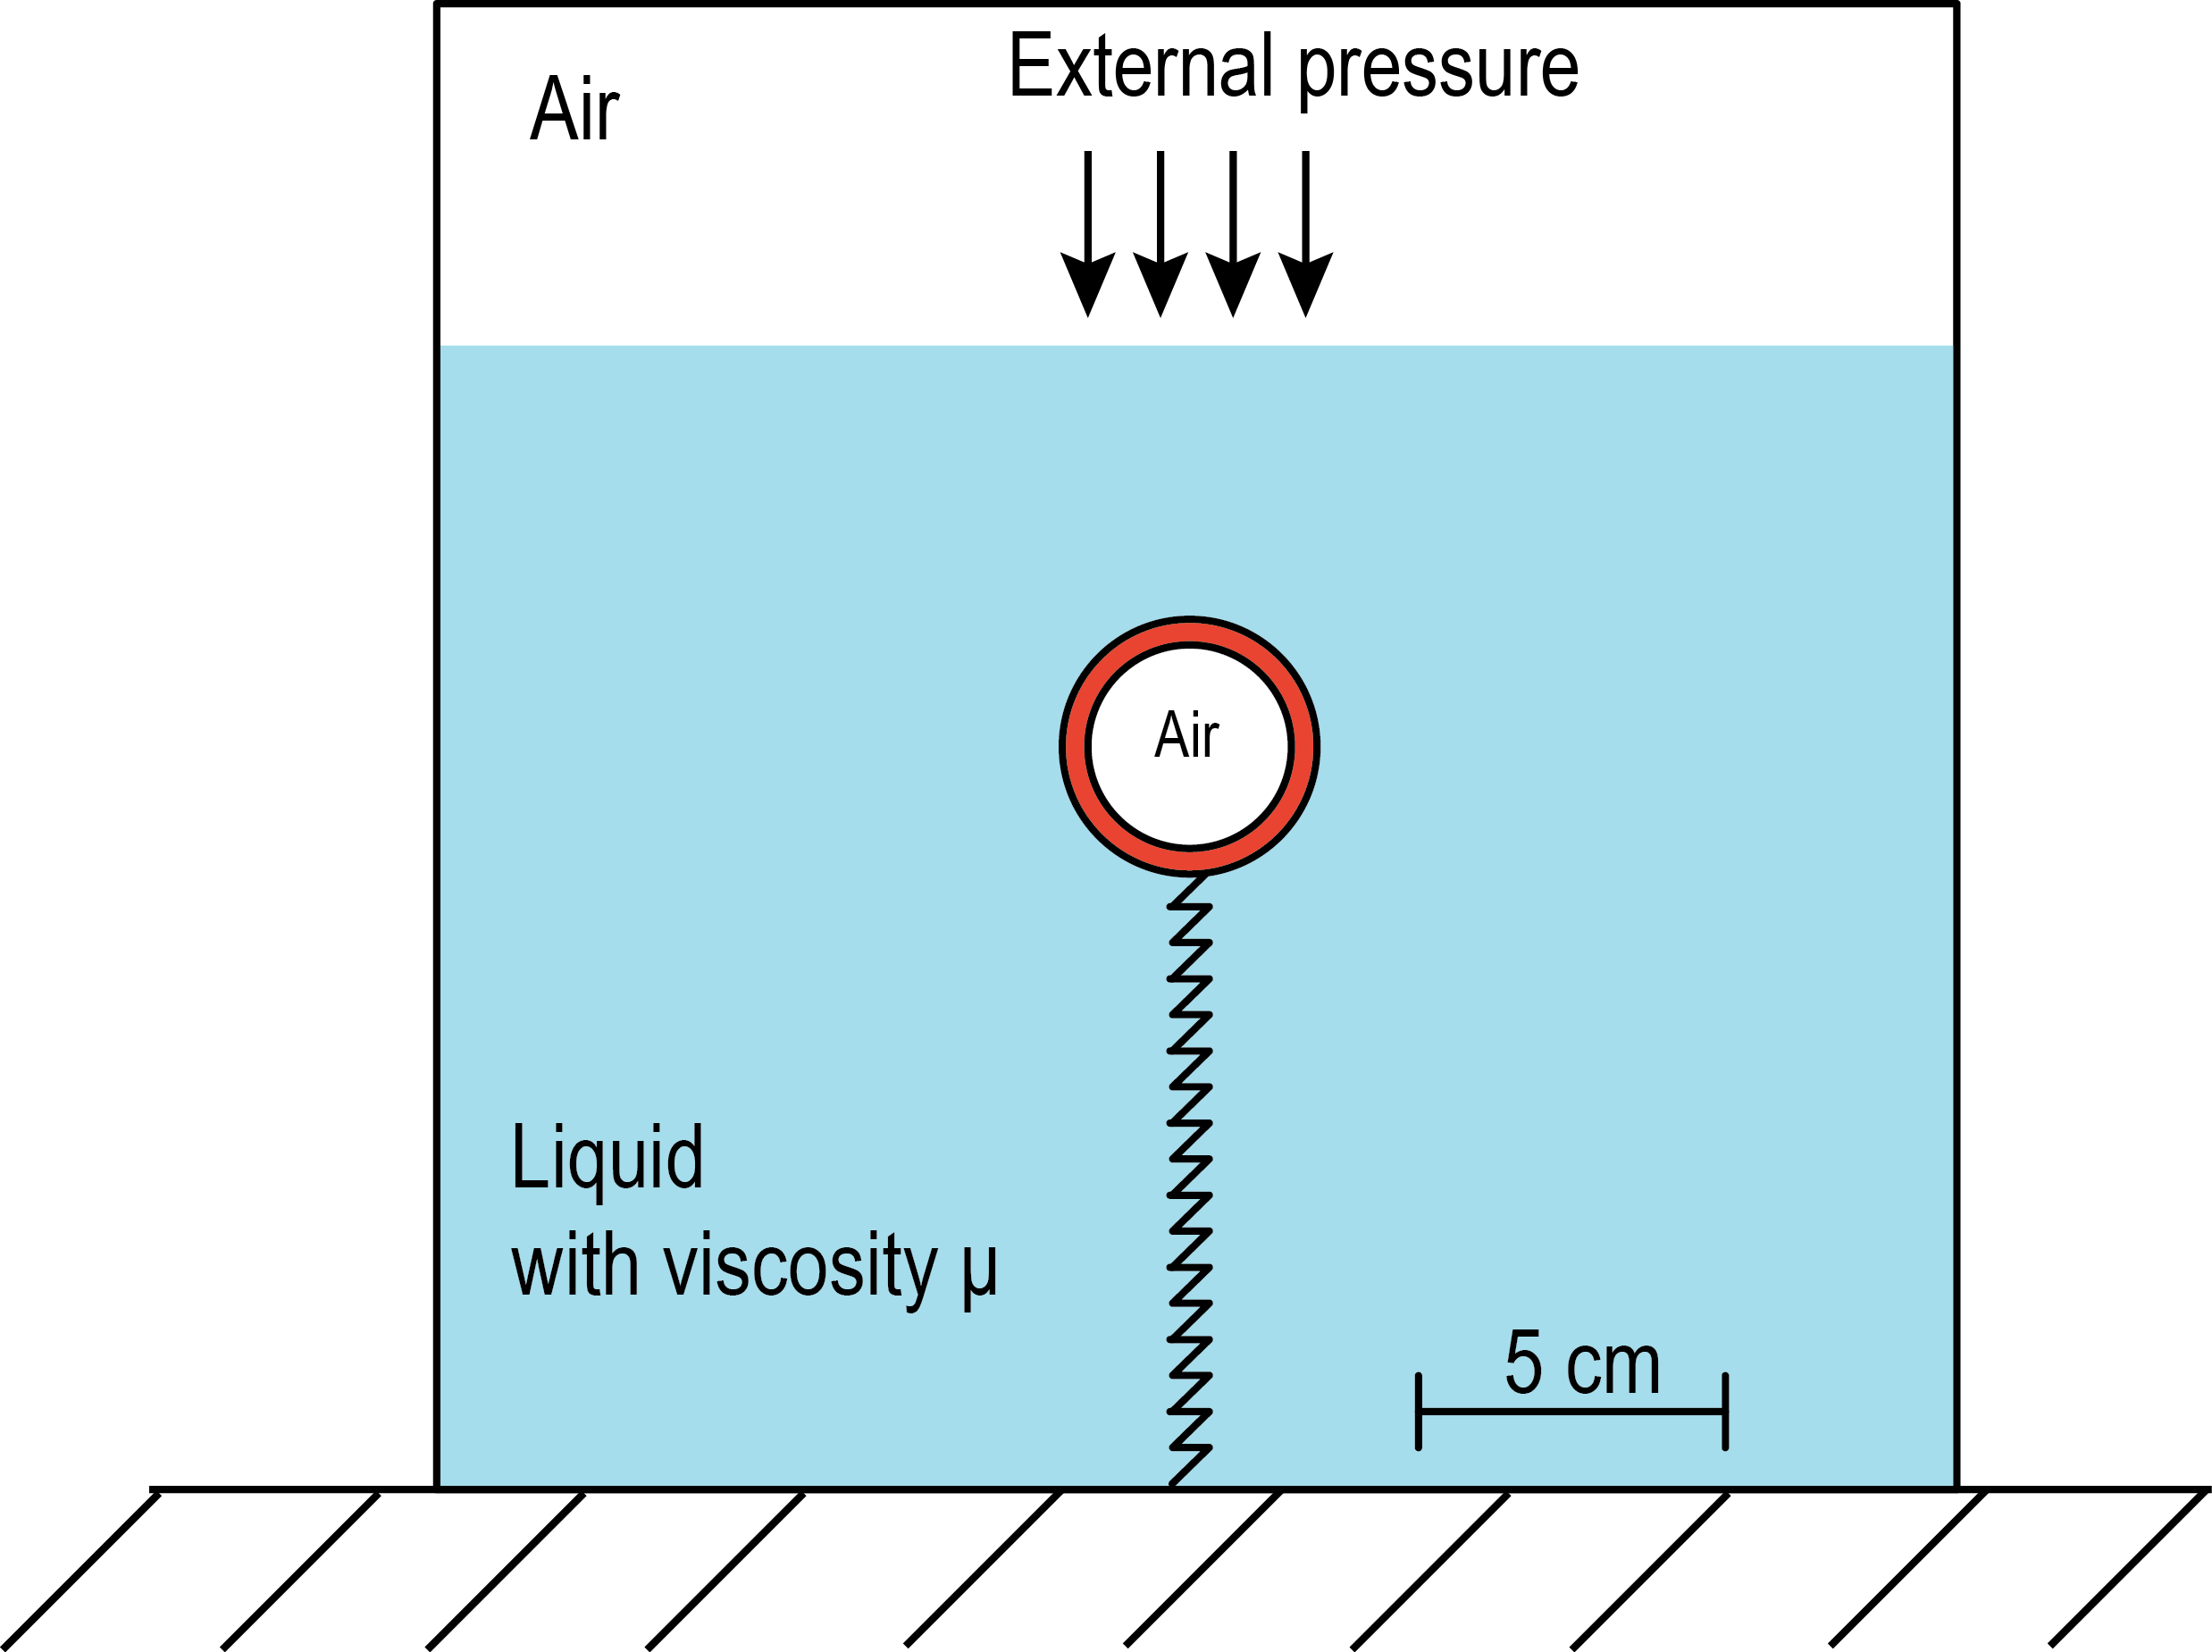
\includegraphics[width=0.73\textwidth]{figures/Chapter_1/schematic_experimental_setup.png}
	\caption{Schematics of the spring experiment}
	\label{fig:spring_experiment_schematic}
\end{figure}

\subsection{Equipment}
\subsubsection{Tank}
\paragraph{}
It consists of a cubic tank (see fig.\ref{fig:tank}) made of anodized Aluminum supplied with windows made of polycarbonate polymer. It is dimensioned to withstand an absolute pressure of $3 10^5 Pa$. Its dimensions are consistent with the non-confinement conditions ***(CITATION)*** where the characteristic length of the container is close to 10 times the characteristic length of the object to be studied.
\begin{figure}[H] %
	\centering%
  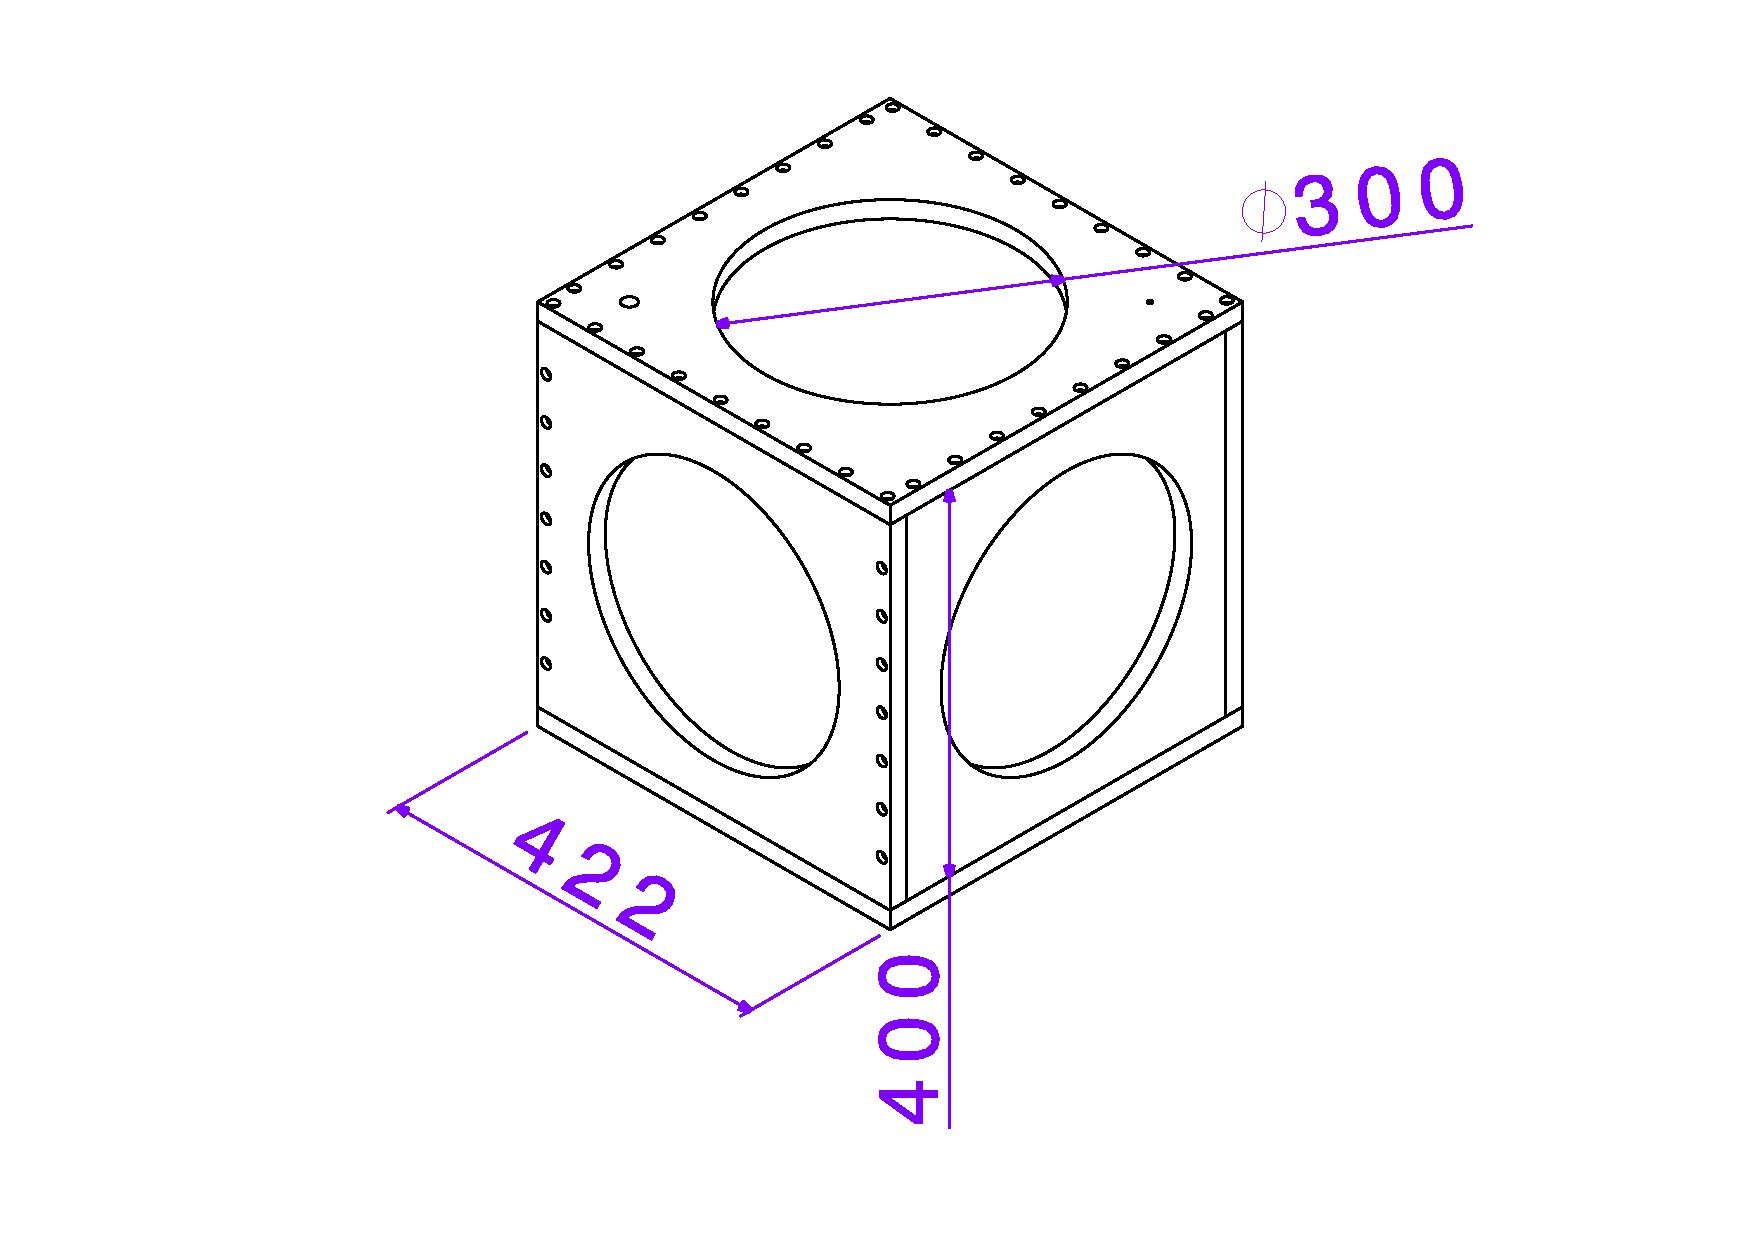
\includegraphics[width=0.73\textwidth]{figures/Chapter_1/cuve.pdf}
	\caption{Schematics of the pressurizeable tank}
	\label{fig:tank}
\end{figure}
\subsubsection{Spring}
\paragraph{}
As described earlier, the spring is used as a force sensor. 
When the system "`shell-spring"' is static, its elongation is directly proportional to the tension force $K \Delta x$, where k is the stiffness coefficient. In the case of our study, the spring is solicited in traction\footnote{At any moment, during the experiment, the elongation of the spring is bigger than the length at rest with no mass attached.}. 
The spring also allows to keep the spherical shell immersed in the liquid.
\paragraph{}
Taking into account that the outer radius for all the capsules studied was fixed at 25 mm and that the buoyancy force is significantly larger than the weight, only one spring stiffness was needed to carry out the experiment.
The spring-shell system was dimensioned to have a total length of 200 mm, at rest, in water. Knowing that after the buckling, the equilibrium state reached is lower due the decrease in volume (by $\approx 20\%$, determined by preliminary results), a constraint was added to avoid the case where the spring rings would be in contact with each other which would bias the force measurement.
\paragraph{}
The characteristics provided by the manufacturer concerning the spring used in this experiment are:
\
\begin{itemize}
	\item Stiffness coefficient : 7 N/m
	\item Length at rest : 100 mm 
	\item Material : EN 10270-3 stainless steel
	\item Wire diameter : 0.5 mm
	\item External diameter: 7.93 mm
\end{itemize}

It was also provided with threaded ends to fit M6 and M4 screws. The M6 end is designed to link the spring to a fixed base at the bottom of the tank. The M4 end is designed to support a suction cup provided with a M4 screw. This suction cup is used to attach the spherical capsule to the spring.




\subsubsection{Pressure controller}
\label{sssection:pressure_controller}
\paragraph{}
Since deflation and re-inflation cycles of the shell are actuated by applying a difference of pressure between the inside of the shell and outside, it was necessary to use a pressure controller.
\paragraph{}
%A pressure controller is not an air compressor, it needs a high pressure input. The user sets the pressure wanted using a piece of software which in turn, communicates with the hardware assigning the desired command. The pressure controller then, opens its valves and regulates the in/out air flux until the desired pressure is reached, using a pressure sensor which measures a relative pressure to the reference: the room atmospheric pressure.
A pressure controller is an instrument that allows to regulate pressure set by the operator in an enclosed environment.
\paragraph{}
The equipment used during this experiment is the OB1 flow control system manufactured by Elveflow\textcopyright. This system is supplied with channels which operate between 0 and 2 bars (relative pressure) and one channel operates between -1 and 1 bar and requires a vacuum pump to reach -1 bar, in addition to a pressure source.
In the spring experiment, the external pressure is the control parameter, therefore only a 0-2 bar channel was used.
\paragraph{}
The pressure is controlled thanks to a graphical interface, which allows to apply different kind of pressure signals such as: constant, ramp, sinusoidal, square signals. It also allows programing sequences using the previously stated signals, but also wait time, triggers and loops. This particular function was helpful to implement reproducible pressure cycles during the spring experiment
\footnote{
This pressure controller is not supposed to be used in such conditions, operating on rather large air volumes. One of its inconveniences was its time response with a max air-flux dimensioned for micro-fluidic experiments. We bought a pressure controller intended to work with large volumes but it was not supplied with neither any power supply nor any software and necessary electronics to control it with a computer. The fact that we were not investigating the actuation frequency role in the physics and the impossibility to control negative relative pressures, comforted us into using the plug and play solution "`OB1"'.}.
%\paragraph{}
%To ensure the proper functioning of the pressure controller, two air filters were used: one upstream, to filter the air between the pressured air supply and the "`OB1"' and one downstream to filter the air between the "`OB1"' and the tank, where liquid vapor can affect the equipments of the "`OB1"' during the pressure regulation phase.
%The air filter used consist in a 5$\mu$m pore size pneumatic filter which removes liquid and solid contaminants. It is supplied with drain that can be opened as needed to drain condensed contaminants.



\subsubsection{Camera,lenses and light sources}
\label{sssection:CLLS}
\paragraph{Camera:}
Taking into account the fast nature of the instability, where the shells undertakes a deformation of almost a radius, in less than 5 ms, it was necessary to use a high-speed camera.
The camera used for this purpose is the Phantom\textcopyright Miro 310, its main characteristics are the following:
\begin{itemize}
	\item Resolution: One megapixel, 1280x800.
	\item Full resolution speed: 3260 frame per second (FPS).
	\item Sensor: CMOS sensor with 20 $\mu$m pixel size, 12-bit depth gray-scale colors.
\end{itemize}
\paragraph{}
It is supplied with a software which allows the control of these parameters and also triggering and storing images.
\paragraph{Lenses:}
A lens with high iris opening value is necessary to capture images at high speed with low light exposure. It was necessary to capture a large field which contains an object of 50 mm plus part of a spring which moves during the process. This is why a fixed focal length $f= 50$ mm with a maximum aperture of f/1.4 was selected.

\paragraph{Light source:}
Three parameters were to take into account for the choice of light sources:
\begin{enumerate}
	\item A stable source of light with no variation of light intensity was required to be able to use the 2D image registration algorithm "`UnwrapJ"', to correct the deformation of the tank windows, due to pressure.
	\item A powerful intensity is required to be able to record at high speed.
	\item A homogenous light source is needed to be able to correctly extract the edges of the shell from the images (no light gradient).	
\end{enumerate}
To do so, two 30x30 daylight balanced led-based panels were used providing 6560 lumen, disposed as shown in figure \ref{fig:schematics_spring}. The one at the back is tuned at full power to highlight the complete ball-spring system and a filter is added to diffuse light and avoid seeing the individual leds. The one upfront is used with 25\% of its power, in order to see the concavity, once the shell is buckled.
\begin{figure}[H] %
	\centering%
  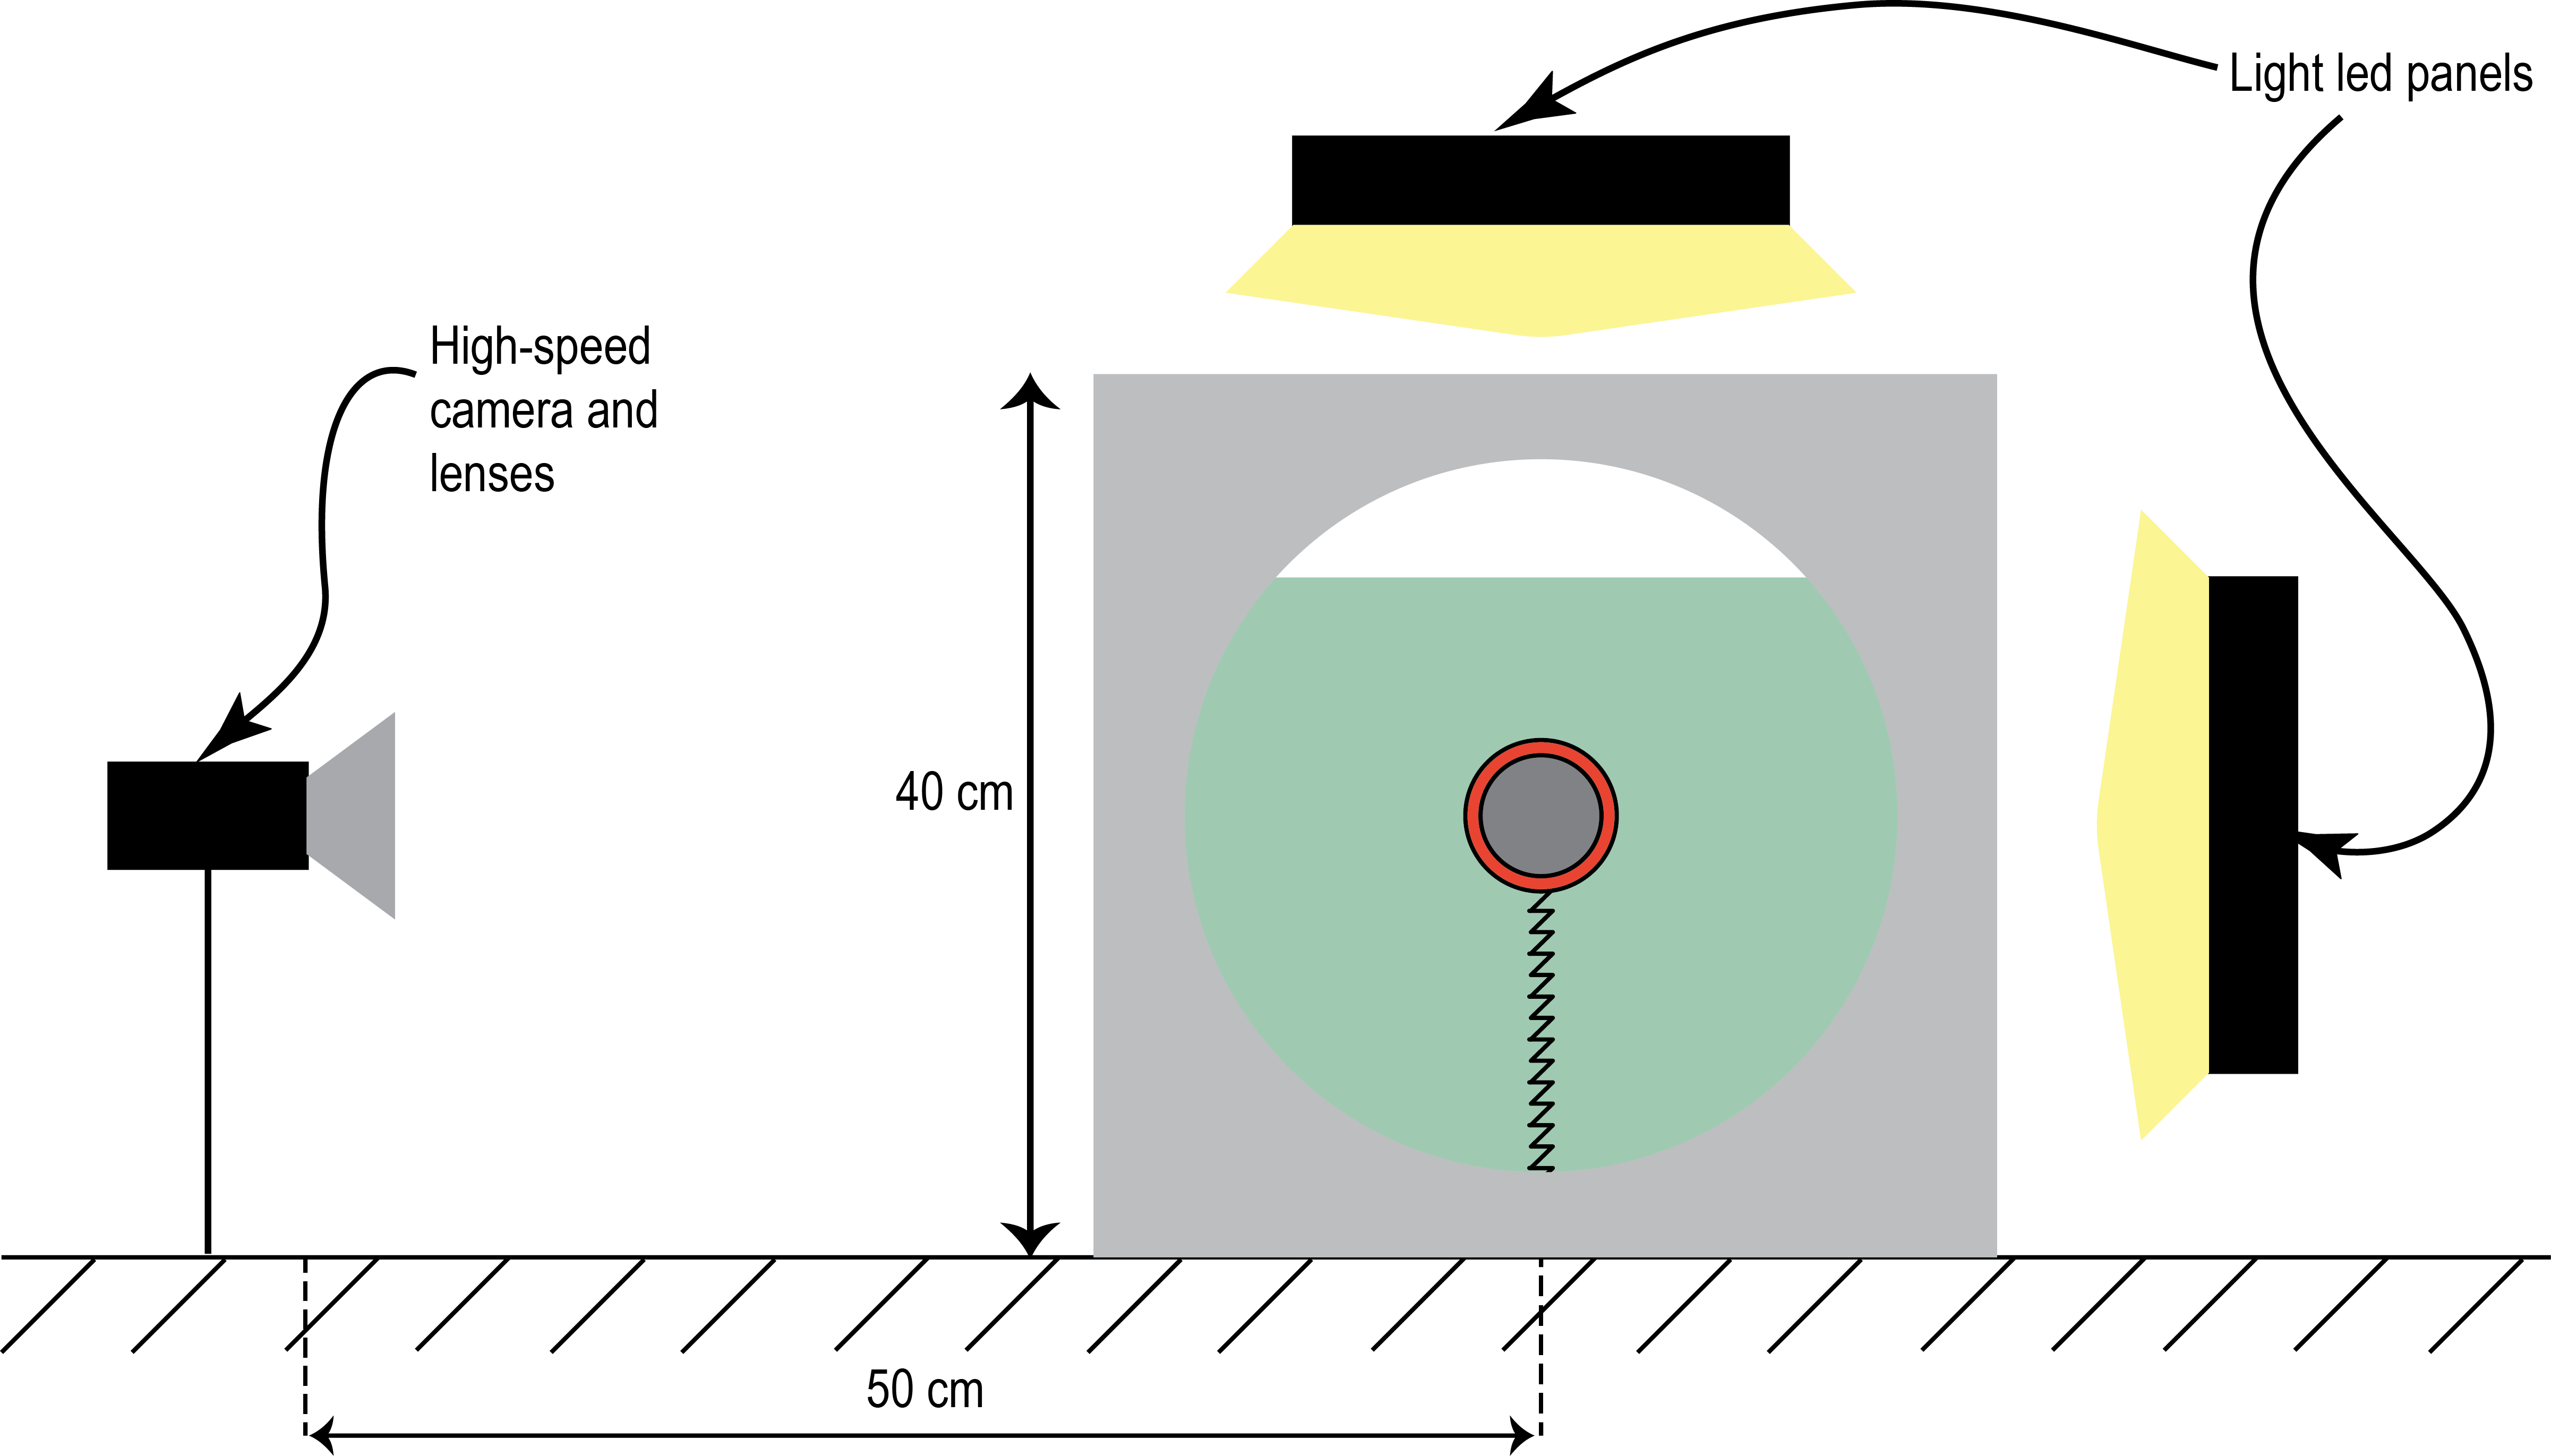
\includegraphics[width=0.73\textwidth]{figures/Chapter_1/schematic_experimental_setup_light_lenses.png}
	\caption{Representation of the light and camera disposition for the spring experiment}
	\label{fig:schematics_spring}
\end{figure}
\newpage
\subsection{Experimental process}
\subsubsection{1-D orientation}
\paragraph{}
Theoretically, the buckling instability nucleates randomly  on the surface of the shell. Practically, this instability always occurs at a specific spot of the elastic shell which represent its weak spot, when the boundary conditions are not changed \footnote{Experimentally, when the shell is in contact of a wall, the buckling spot occurs at the contact point, due to some change in the shell stress.}.
\paragraph{}
To properly conduct a force measurement, using a spring, it is necessary to align the buckling spot in the spring axis to obtain a 1-D displacement. To do so, a series of preliminary experiments are conducted to determine precisely the buckling spot:
First, mark the shell surface with 12 distinctive symbols, then put the marked ball inside the tank and apply a pressure to induce the buckling instability. Once buckled, define the closest symbol to the concavity center resulting from the buckling. Link the shell to the suction cup fixed on the spring, in a way to have the buckling spot aligned to the spring and mark the position of the guessed buckling spot and the attaching area and pressurize the the tank to trigger the buckling again. Measure the angle between the spring axis and the concavity and repeat the operation until a 90° angle is achieved. 
\paragraph{}
This step also allows to determine the experimental critical pressure at which the buckling and unbuckling occur.
\subsubsection{Experimental protocol}
\paragraph{}
We used three fluids in this experiment, and in each fluid, three capsules were investigated varying the relative thickness $\frac{d}{R}$ (see sec.\ref{sec:Spherical_shells}).
The main characteristics of the fluids used are shown in table \ref{tab:fluid_carac_spring}. 
\begin{table}[H]
	\centering
		\begin{tabular}{|l|c|r|}
			\hline
			Fluid & Density (Kg.m$^{-3}$) & Viscosity (Pa.s)\\
			\hline
			Glycerol & 1250 & 1 \\
			\hline
			Water & 1000 & 10$^{-3} $\\
			\hline
			Air &  1.2 & 10$^{-6}$\\
			\hline
		\end{tabular}
	\caption{Fluids used in the experiments and their main properties at room temperature.}
	\label{tab:fluid_carac_spring}
\end{table}
The following experimental protocol is applied for each fluid.
%\paragraph{Quasi-static experiments:}
%We noticed, during the first experiments done with the spring that the shape of a shell submitted to a constant pressure P, continues to slightly evolve in time due to the relaxation of the material through creep. To investigate the relevance of this effect on the buckling/unbuckling dynamics, quasi-static experiments were conducted by submitting the shell to a pressure cycle which evolves at a slow rate. Practically, a step-like cycle was applied knowing the buckling and unbuckling critical pressures.\\
%Figure \ref{fig:quasi_static_pressure_cycle} shows a qualitative example of such step-like cycle where the step width represents the amount of time waited at each pressure step\footnote{by varying this step width, we can evaluate its importance and how it impacts the instability dynamics}.
%First, an image is recorded at (P=0), then the pressure is increased by a pressure step and is kept constant during a time $T=step width$, at the end of this time an image is recorded. This process is repeated until nearing the pressure at which the buckling occurs which can slightly vary from an experiment to another, the pressure is then gradually increased by smaller steps\footnote{The smaller steps are necessary in order to keep the pressure constant at the buckling and unbuckling phases, to independently study the buckling and unbuckling dynamics.}
 %and when arriving to a critical pressure where the buckling occurs, the camera is triggered and a movie is recorded at 5000 FPS \footnote{Figure \ref{fig:quasi_static_pressure_cycle} shows a longer time at the buckling and unbuckling phases to count for the time necessary to save the resulting movies, which takes about 8 minutes}. An image is taken at the end of the buckling phase, in order to record the state to which the capsule has relaxed to, following the buckling.
%The pressure is decreased following the same procedure until nearing the critical pressure at which the unbuckling occurs and the same procedure is followed for the buckling phase. After that, the pressure is decreased until reaching zero.
%This protocol is performed for each step width, and there are 2 of them: 10 minutes and 1 minute. 10 minutes, represents the time after which the final state of relaxation is reached and any change that might occur cannot be perceived within our experimental precision. This limit is specific to the material used. The 1 minute time was added to measure the rate at which this relaxation happens.\\
   
%\begin{figure}[H] %
	%\centering%
  %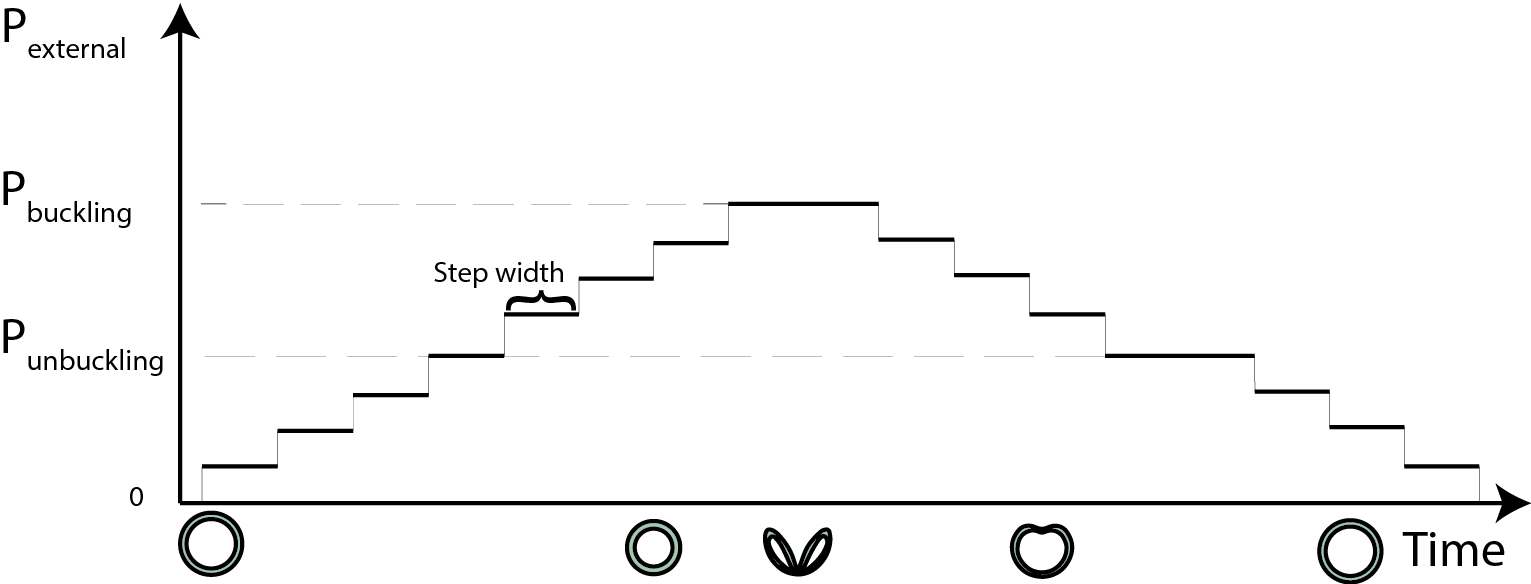
\includegraphics[width=\textwidth]{figures/Chapter_1/quasi_static_pressure_cycle.png}
	%\caption{Qualitative representation of pressure cycles applied for the quasi-static experiments}
	%\label{fig:quasi_static_pressure_cycle}
%\end{figure}
\paragraph{Dynamic experiments:}
%In the second set of experiments, step width is shortened to 20 seconds\footnote{Time necessary to save images to the computer.}, and a similar cycle is applied with the exception of the phase between buckling phase and the unbuckling phase where the depressurization rate was varied, to investigate the production of thrust during the rolling. 
Figure \ref{fig:dynamic_pressure_cycle} shows a qualitative example of a pressure cycle applied during the experiments. The parameter $\alpha$ corresponds to the depressurization rate to get from the buckling pressure to near the unbuckling pressure. Three different rates are applied.
First, an image is recorded at (P=0), then the pressure is increased by a pressure step  and an image is recorded. This process is repeated until nearing the pressure at which the buckling occurs which can slightly vary from an experiment to another, the pressure is then gradually increased by smaller steps\footnote{The smaller steps are necessary in order to keep the pressure constant at the buckling and unbuckling phases, to independently study the buckling and unbuckling dynamics.}
 and when arriving to a critical pressure where the buckling occurs, the camera is triggered and a movie is recorded at 5000 FPS. An image is taken at the end of the buckling phase, in order to record the state to which the capsule has relaxed to, following the buckling.
The pressure is decreased with a certain depressurization rate until nearing the critical pressure at which the unbuckling occurs and the same procedure is followed for the buckling phase. After that, the pressure is decreased until reaching zero.

\begin{figure}[H] %
	\centering%
  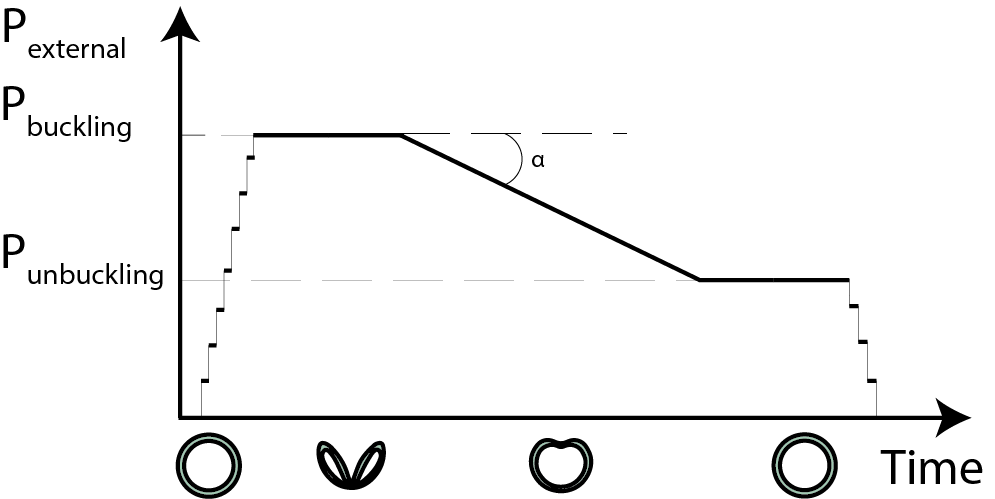
\includegraphics[width=\textwidth]{figures/Chapter_1/dynamic_pressure_cycle.png}
	\caption{Qualitative representation of pressure cycles applied during the experiments}
	\label{fig:dynamic_pressure_cycle}
\end{figure}
The fluid temperature is measured at the beginning of the pressure cycle and at its end. These temperature measurements are then, used to properly characterize the viscosity of the medium, by taking a sample and perform rheological measurements, thanks to a rheometer.\\
The tables \ref{tab:Experimental_pressure_cycle_parameters_in_glycerol},\ref{tab:Experimental_pressure_cycle_parameters_in_water} and \ref{tab:Experimental_pressure_cycle_parameters_in_air} summarize the control parameters of the pressure cycle for each $\frac{d}{R}$, in each fluid.
\begin{table}[H]
	\centering
		\begin{adjustbox}{width=\textwidth}
			\begin{tabular}{|c|c|c|c|c|}
				\hline
				Capsules & Buckling pressure (mbar) & Unbuckling pressure (mbar) & Depressurization rates (mbar.s$^{-1}$) & Temperature (Celsius) \\
				\hline
				$\frac{d}{R} = 0.08$ & 100 & [70,80] & -1, -10, -20 & [20,21.5]\\
				\hline
				$\frac{d}{R} = 0.22$ & [780,790] & [380,390] & -1, -10, -15 & [24.5,26]\\
				\hline
				$\frac{d}{R} = 0.30$ & [1350,1450] & [620,660] & 100 mbar steps, -1, -10 & [25,26]\\
				\hline
			\end{tabular}
		\end{adjustbox}
	
	\caption{Experimental pressure cycle parameters in glycerol}
	\label{tab:Experimental_pressure_cycle_parameters_in_glycerol}
\end{table}

\begin{table}[H]
	\centering
		\begin{adjustbox}{width=\textwidth}
			\begin{tabular}{|c|c|c|c|c|}
				\hline
				Capsules & Buckling pressure (mbar) & Unbuckling pressure (mbar) & Depressurization rates (mbar.s$^{-1}$) & Temperature (Celsius) \\
				\hline
				$\frac{d}{R} = 0.08 $ & [100,110]& [75,85] & -1, -10, -20 & [23,23.5]\\
				\hline
				$\frac{d}{R} = 0.22$ & 780 & [360,370] & -1, -10, -20 & [20,23.2]\\
				\hline
				$\frac{d}{R} = 0.30$ &  \multicolumn{4}{c|}{Experiments were not possible due to the non visibility of the buckling concavity in water.}\\
				\hline
			\end{tabular}
		\end{adjustbox}
	
	\caption{Experimental pressure cycle parameters in water}
	\label{tab:Experimental_pressure_cycle_parameters_in_water}
\end{table}

\begin{table}[H]
	\centering
		\begin{adjustbox}{width=\textwidth}
			\begin{tabular}{|c|c|c|c|c|}
				\hline
				Capsules & Buckling pressure (mbar) & Unbuckling pressure (mbar) & Depressurization rates (mbar.s$^{-1}$) & Temperature (Celsius) \\
				\hline
				$\frac{d}{R} = 0.08$ & [100,110]& [70,80] & -1, -1, -2 & [23.5,25]\\
				$\frac{d}{R} = 0.22$ & [850,900] & [380,480] & -1,-2,-2.5 & [24.5,26]\\
				$\frac{d}{R} = 0.30$ & 1570 & 790 & -1 & 23 \\
				\hline
			\end{tabular}
		\end{adjustbox}
	\caption{Experimental pressure cycle parameters in air}
	\label{tab:Experimental_pressure_cycle_parameters_in_air}
\end{table}







\subsection{Image treatment}
\paragraph{}
 The image treatment is the basis of the measurements extracted from the spring experiment, since every physical quantity of interest is extracted from the images. But before extracting these quantities from the images, a correction of the windows distortion due to the pressurization of the tank was necessary.
\subsubsection{Image calibration due to window distortion}
\paragraph{Distortion correction:}
When static pressure is applied inside the tank used for the experiment, its windows made out of polycarbonate, bend. This bending creates a sort of a barrel distortion which depends on the pressure applied inside the tank (fig.\ref{fig:barrel_distortion}). This distortion alters the images recorded during the experiment and ultimately any distance measurements extracted from them. This error depends on the camera position in regard to the window, the spring-ball position in regard to the window and the pressure inside the tank.For example, an estimation of this deformation at (P = 1000 mbar), by measuring a horizontal central line between the image at (P=0) and at (P=1000 mbar) yields an elongation of $\epsilon_{horizontal} = \frac{\Delta L}{L_0} = 2\%$
\begin{figure}[H] %
	\centering%
  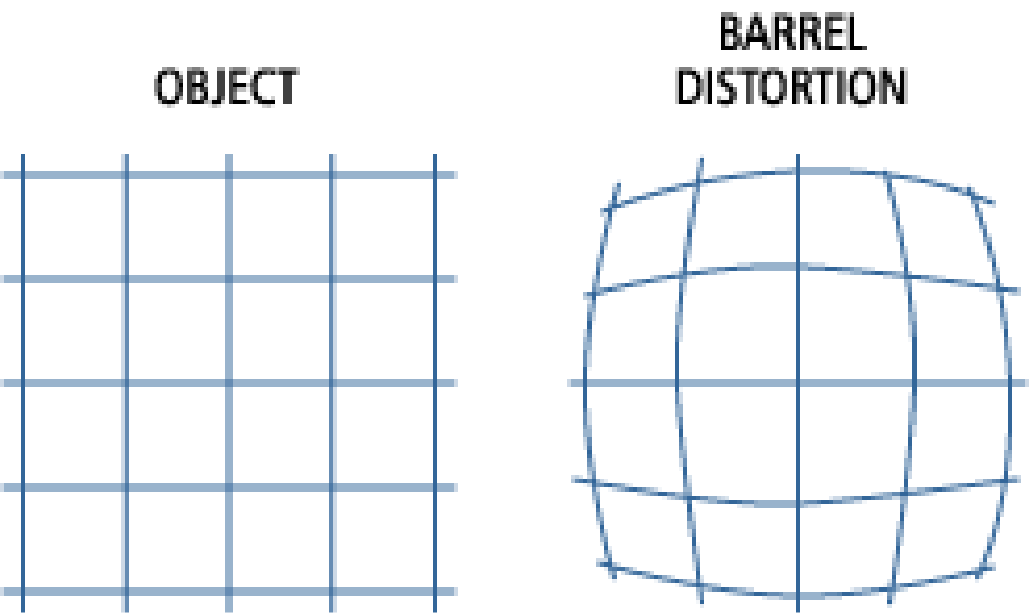
\includegraphics[width=0.48\textwidth]{figures/Chapter_1/barrel_effect.png}
	\caption{Qualitative representation of a barrel distortion}
	\label{fig:barrel_distortion}
\end{figure}
 To correct this effect, numerical method is applied to find the deformation of the image between the rest state where the relative pressure is zero and a state at pressure P. Once found, this deformation matrix is inverted and we can transform a distorted image to a non-distorted one.
To calibrate the correction, the spring-ball system is removed and a damier is placed at the same position as the spring-ball system. Iimages are recorded for each pressure step, used during experiments in one fluid.
 From each damier image, we extracted a deformation matrix that links the rest state at (P=0) to the damier image at (P=p$_{image}$) and the deformation matrix is inverted to get the transformation needed to transform the damier image at (P=p$_{image}$) into the damier image at (P=0), using an algorithm implemented in the registration plugin category of ImageJ, called "`bUnwrapJ"'.
\paragraph{}
"`bUnwarpJ"' is an algorithm for elastic and consistent image registration developed as an ImageJ plugin. It performs a simultaneous registration of two images, A and B. Image A is elastically deformed in order to look as similar as possible to image B, and, at the same time, the "inverse" transformation (from B to A) is also calculated so a pseudo-invertibility of the final deformation could be guaranteed (fig\ref{fig:scheme_bunwrapJ}).

\begin{figure}[H] %
	\centering%
  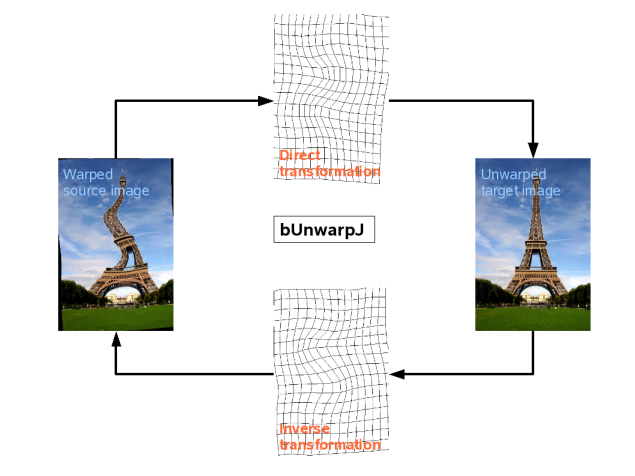
\includegraphics[width=\textwidth]{figures/Chapter_1/BUnwarpJ_scheme.png}
	\caption{Illustration of the bUnwarpJ algorithm principle}
	\label{fig:scheme_bunwrapJ}
\end{figure}

This image registration algorithm is based on the minimization of an energy functional that includes the dissimilarity between the source and target images -in both directions- $E_{img}$, an optional landmark constraint $E_{\mu}$, a regularization term $(E_{div} + E_{rot})$, and an energy term $E_{cons}$ that accounts for the geometrical consistency between the elastic deformation in both directions. Namely, the energy function is given by:
\begin{equation*}
		E = w_iE_{img} + w_{\mu}E_{\mu} + (w_dE_{div} + w_rE_{rot}) + w_cE_{cons} 
\end{equation*}
                  

Where the weights of every term are set by the user in the main window of the plugin. The optimization process is a Levenberg-Marquardt minimization enhanced by a Broyden-Fletcher-Goldfarb-Shanno (BFGS) estimate of the local Hessian of the goal function, and both, images and deformations are represented by cubic B-splines \cite{bunwrapJ,unwrapJ}. 

\paragraph{}
Once the deformation matrix and its inverse extracted from the calibration step, each inverse transformation matrix $A(P)$ is applied to the $image(P)$ recorded during the spring experiment. The resulting image corresponds to an image recorded using a non-deformed tank window.\\
All this process was automatized, using a script written in ImageJ macro language.
\subsubsection{Contour extraction algorithm}
\paragraph{}
Once the distortion corrected, we needed to extract from each image three physical quantities:
\begin{enumerate}
	\item Elongation of the spring.
	\item Shape and volume of the capsule.
	\item Gravity center of the capsule.
\end{enumerate}
\paragraph{}
An algorithm was written in Python, based on an image treatment library called "`Opencv"', to automatically extract the three quantities for each image, following these steps, enriched by illustrations for each step, applied to a raw image, in the buckling state, which represents the most complex  situation (fig.\ref{fig:raw_image}):
\begin{figure}[H] %
	\centering%
  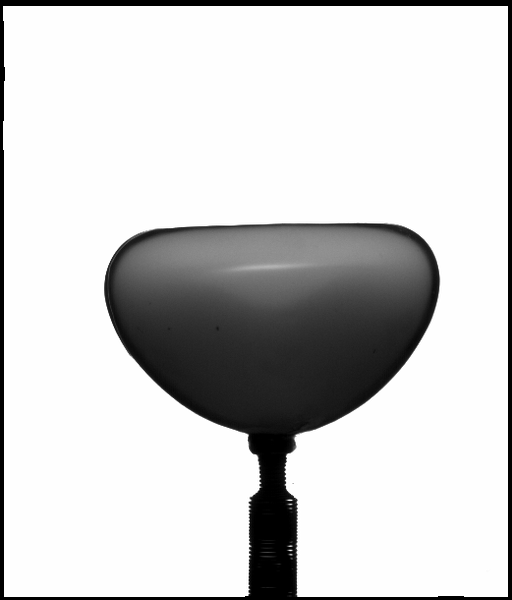
\includegraphics[width=0.48\textwidth]{figures/Chapter_1/raw_image.png}
	\caption{Raw image used for the illustrations}
	\label{fig:raw_image}
\end{figure}
\paragraph{}
First, the image is cropped and filtered, using two types of filters: a Gaussian filter where each point in the input array is convolved with a Gaussian kernel and then summing them all to produce the output array. Gaussian blurring is highly effective in removing Gaussian noise from the image. The second, is a median filter, which runs through each element of the image and replace each pixel with the median of its neighboring pixels. it is highly effective against salt-and-pepper noise in the images.
The filtering kernel size were kept to a low level, to avoid dilatation of the pixels and an alteration of the capsule's contour.

\paragraph{}
Second, Canny edge detector algorithm\cite{canny} is used to find the edges on the image (fig.\ref{fig:canny}). Briefly, this algorithm relies on finding the intensity gradients of the image, thinning the edge, by using the "`non-maximum suppression"' technique, and then applying a double threshold to get rid of the noise.
\begin{figure}[H] %
	\centering%
  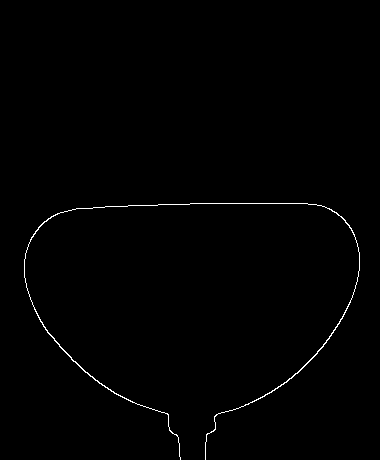
\includegraphics[width=0.48\textwidth]{figures/Chapter_1/canny.png}
	\caption{Canny edge detection}
	\label{fig:canny}
\end{figure}
\paragraph{}
From the canny image (fig.\ref{fig:canny}), the white pixels are extracted, to get the general contour. Then, the capsule shape is extracted, by setting a threshold on the horizontal distance between two white points.

%by first, determining the maximum horizontal distance "`maxD"' between two white points, this distance is close to the maximum width of the ball. Knowing the y-position of "`maxD"', and exploiting the monotonous decrease of the horizontal distance, at higher y (the origin being the top left pixel), we can remove the spring shape by setting a minimum horizontal distance, as shown in figure \ref{fig:ball_shape}.

%\begin{figure}[H] %
	%\centering%
  %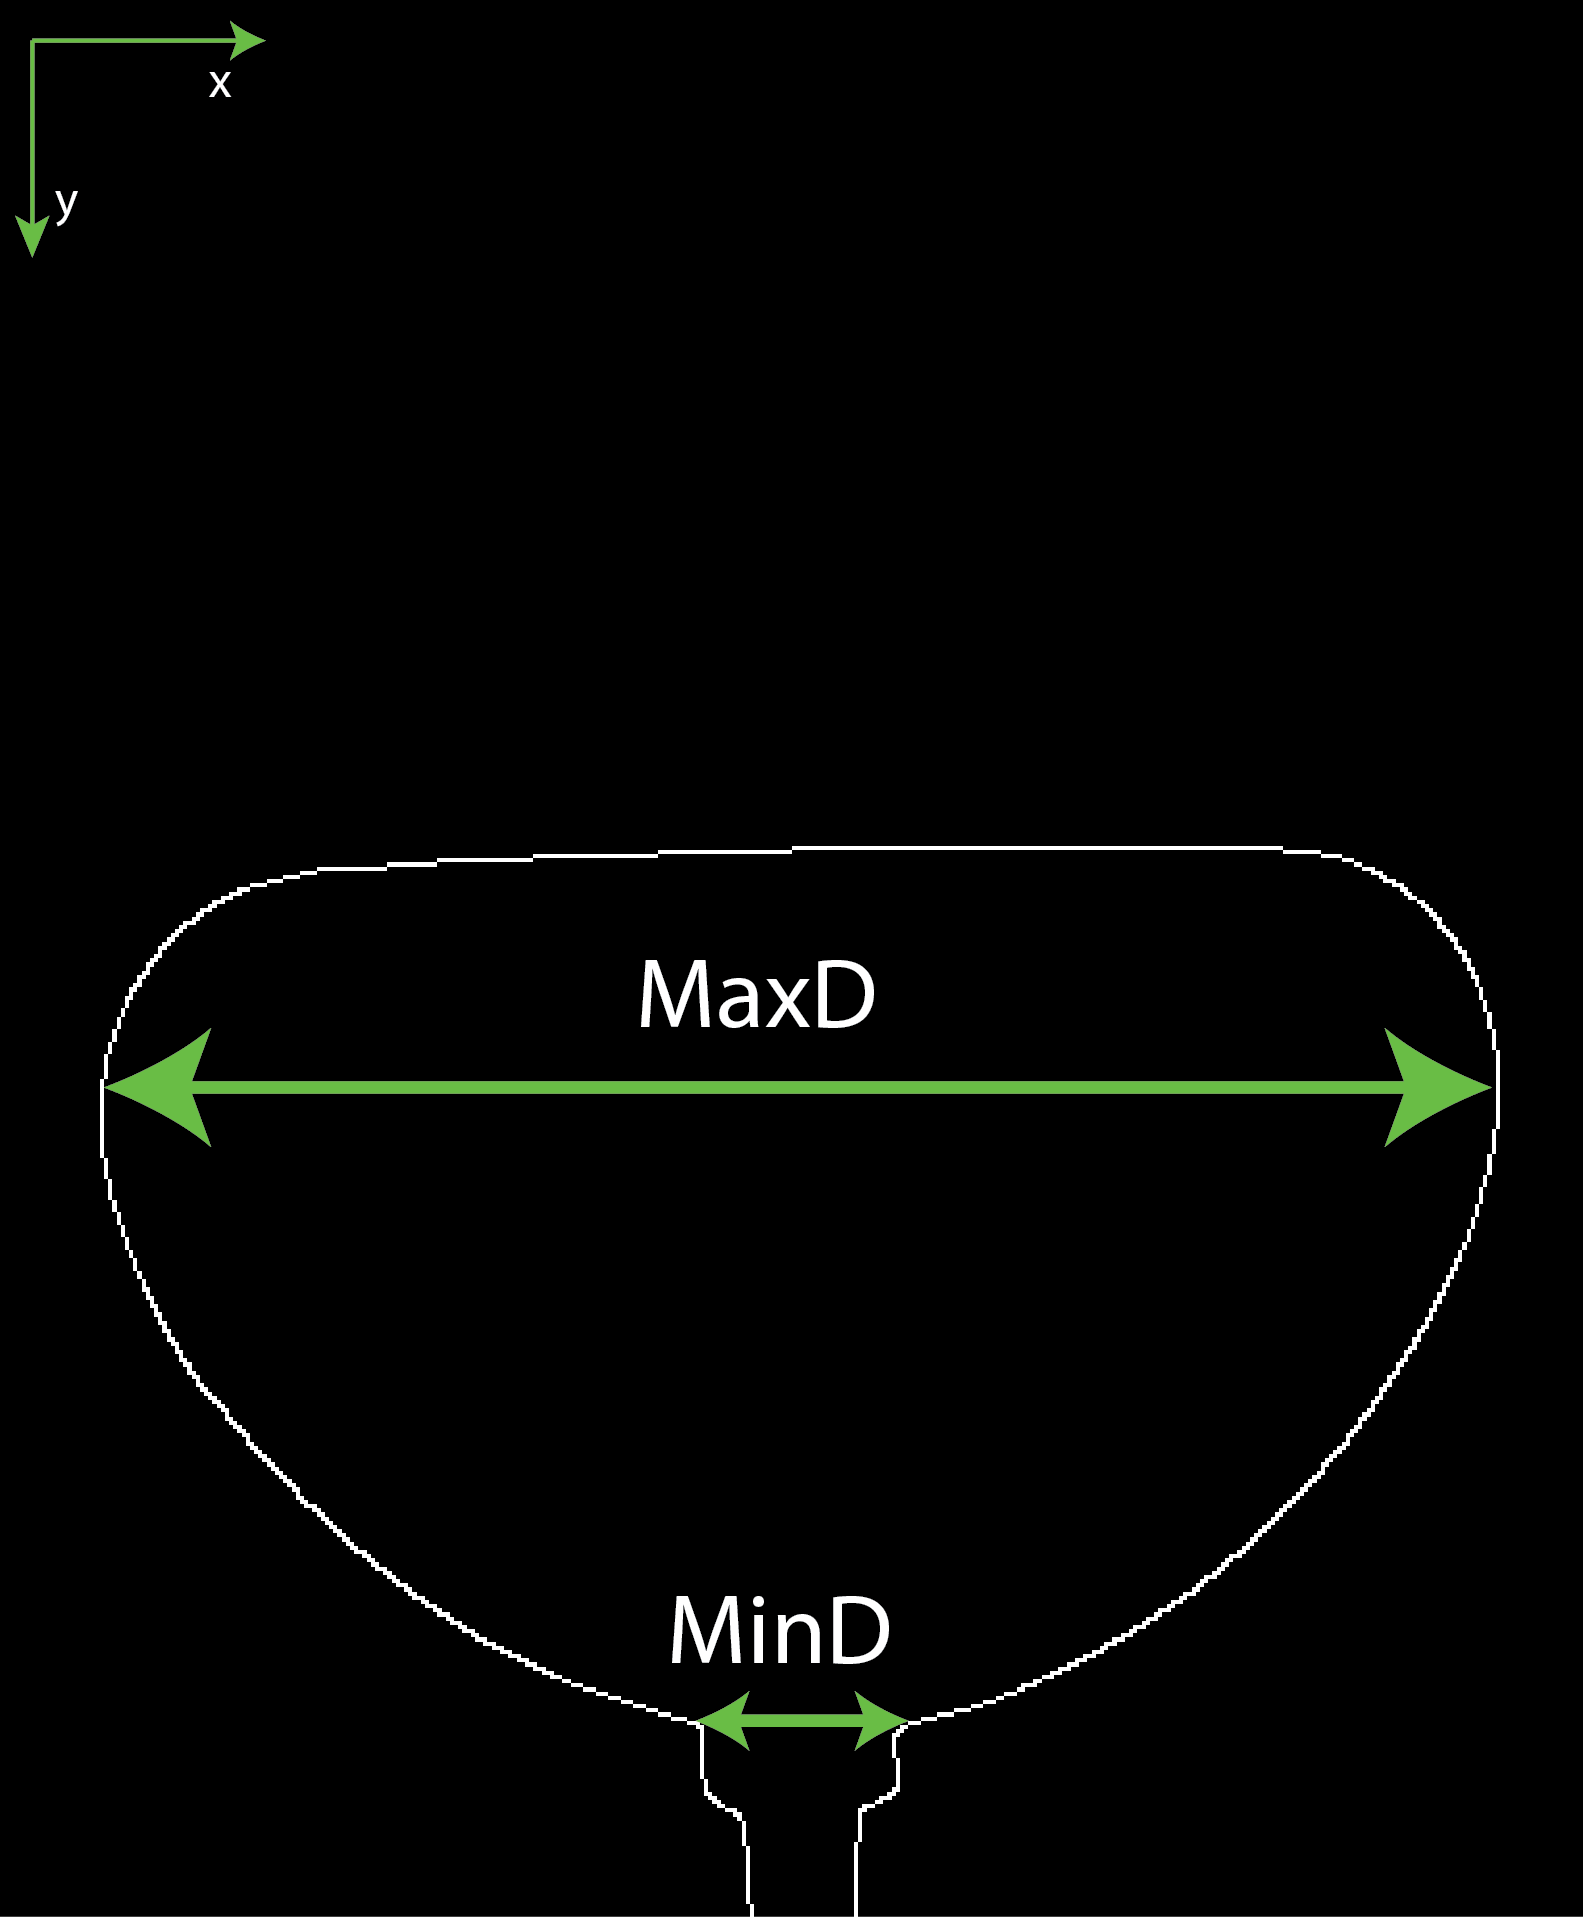
\includegraphics[width=0.48\textwidth]{figures/Chapter_1/ball_shape.png}
	%\caption{Ball shape}
	%\label{fig:ball_shape}
%\end{figure}
\paragraph{}
Once the ball shape defined, its outer contour is fitted with a parametric curve (see fig.\ref{fig:outer_contour}), defined in the polar coordinates system as such: 
\begin{equation*}
	\tilde{R}(\theta)_i =\sum\limits_{k=0}^M a_k \sin(\theta_{exp_i}-\theta_0)^k
	\label{eq:parametric_curve}
\end{equation*}
The algorithm followed can be found in appendix \ref{AppendixA}.
\begin{figure}[H] %
	\centering%
  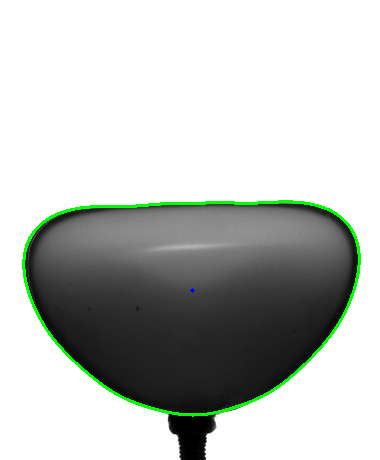
\includegraphics[width=0.48\textwidth]{figures/Chapter_1/outer_contour.png}
	\caption{Fitted outer contour in green, and center of the parametric curve in blue}
	\label{fig:outer_contour}
\end{figure}
\paragraph{}
Once the outer contour fitted (fig.\ref{fig:outer_contour}), the experimental points defining the concavity are extracted from the image automatically. A region of interest (ROI) where the concavity occurs is defined around the maximum diameter region (fig\ref{fig:concavity_extraction}. Canny edge detector, is then applied to the ROI.
\begin{figure}[H] %
	\centering%
  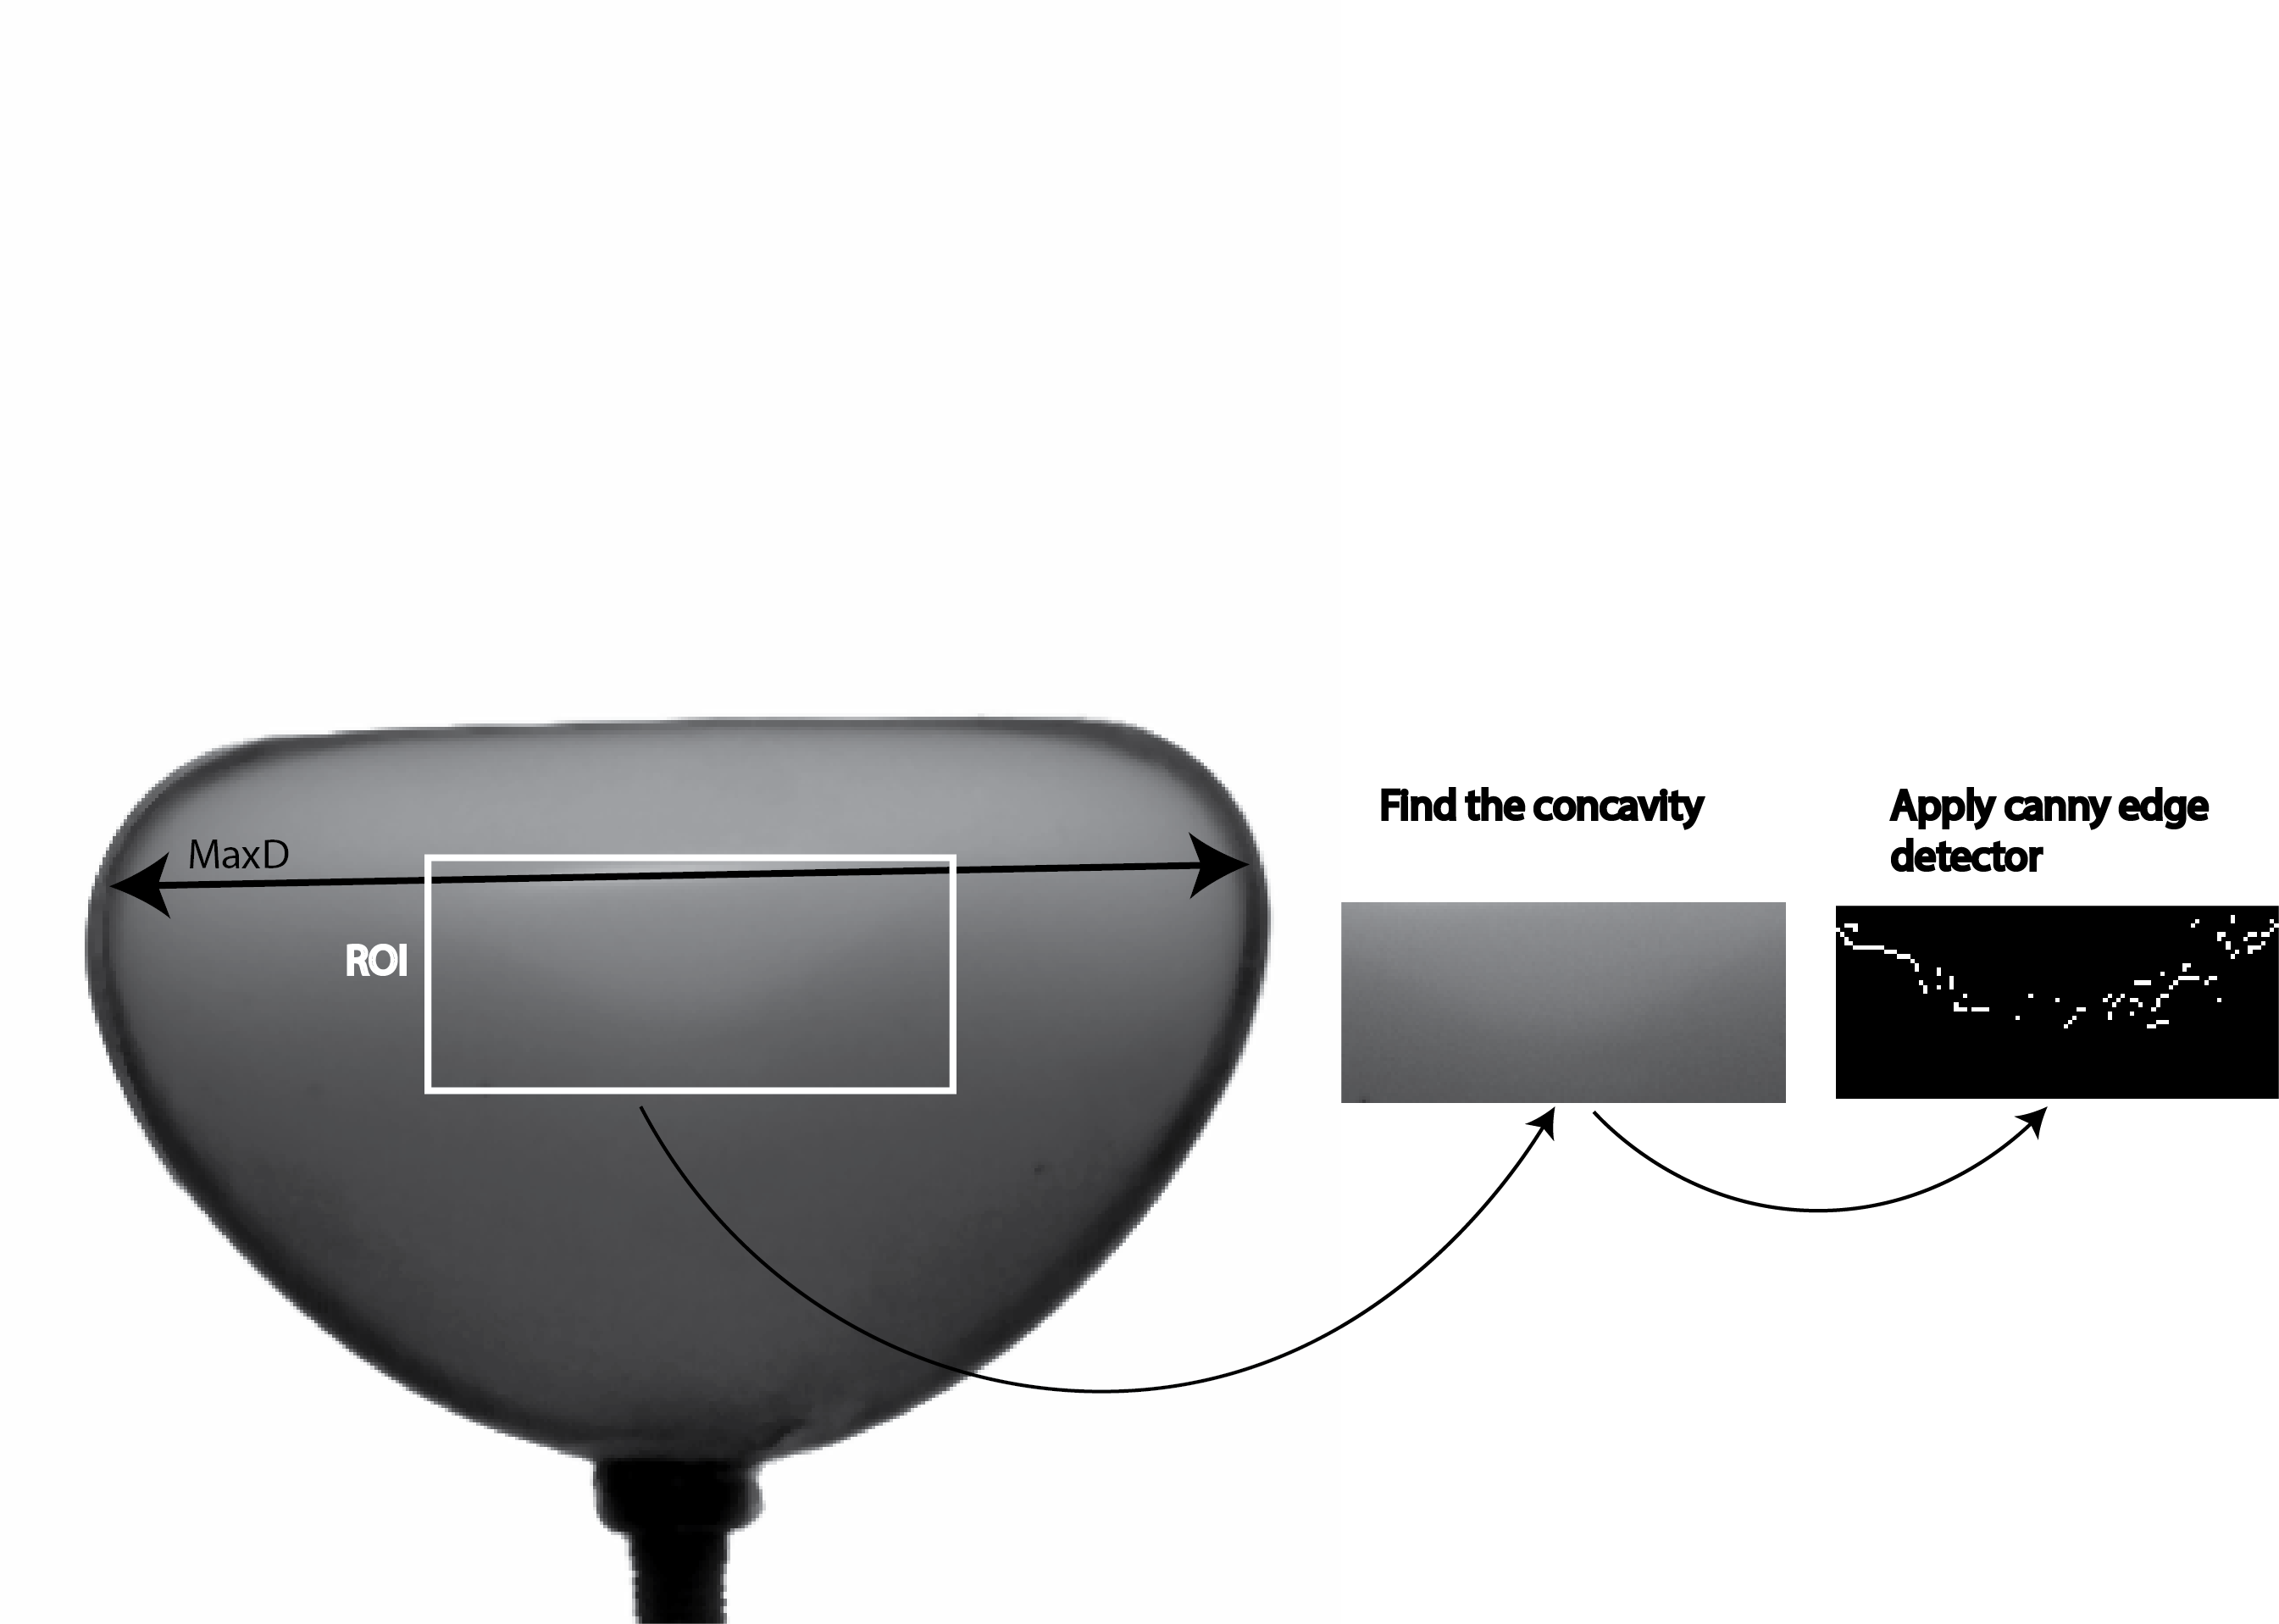
\includegraphics[width=\textwidth]{figures/Chapter_1/concavity_extraction.png}
	\caption{Extraction of the concavity experimental points}
	\label{fig:concavity_extraction}
\end{figure}
\paragraph{}
To create a complete fit between the outer contour and a fit of the concavity, we need first, to cut the outer contour where it ceases to belong to the shape generatrix, which generates the physical surface of the concave capsule, when integrated around the y-axis. This limit is set by the point of the parametric outer curve where the tangent is horizontal.
Practically, it means, find the point $M(R_{h},\theta_h)$, such as the the following condition is respected:
\begin{equation}
	\tan(\theta+\alpha) =0
	\label{eq:tangent_horizontal}
\end{equation}
Where $\alpha$ is the angle defined between the tangent line $T$ with the vector $\vec{OM}$ (see fig.\ref{fig:Illustration_tangent}), such as:
\begin{equation}
	\tan(\alpha) =|{\frac {\tilde{R}(\theta )}{\tilde{R}'(\theta )}}|
	\label{eq:tangent}
\end{equation}
\begin{figure}[H] %
	\centering%
  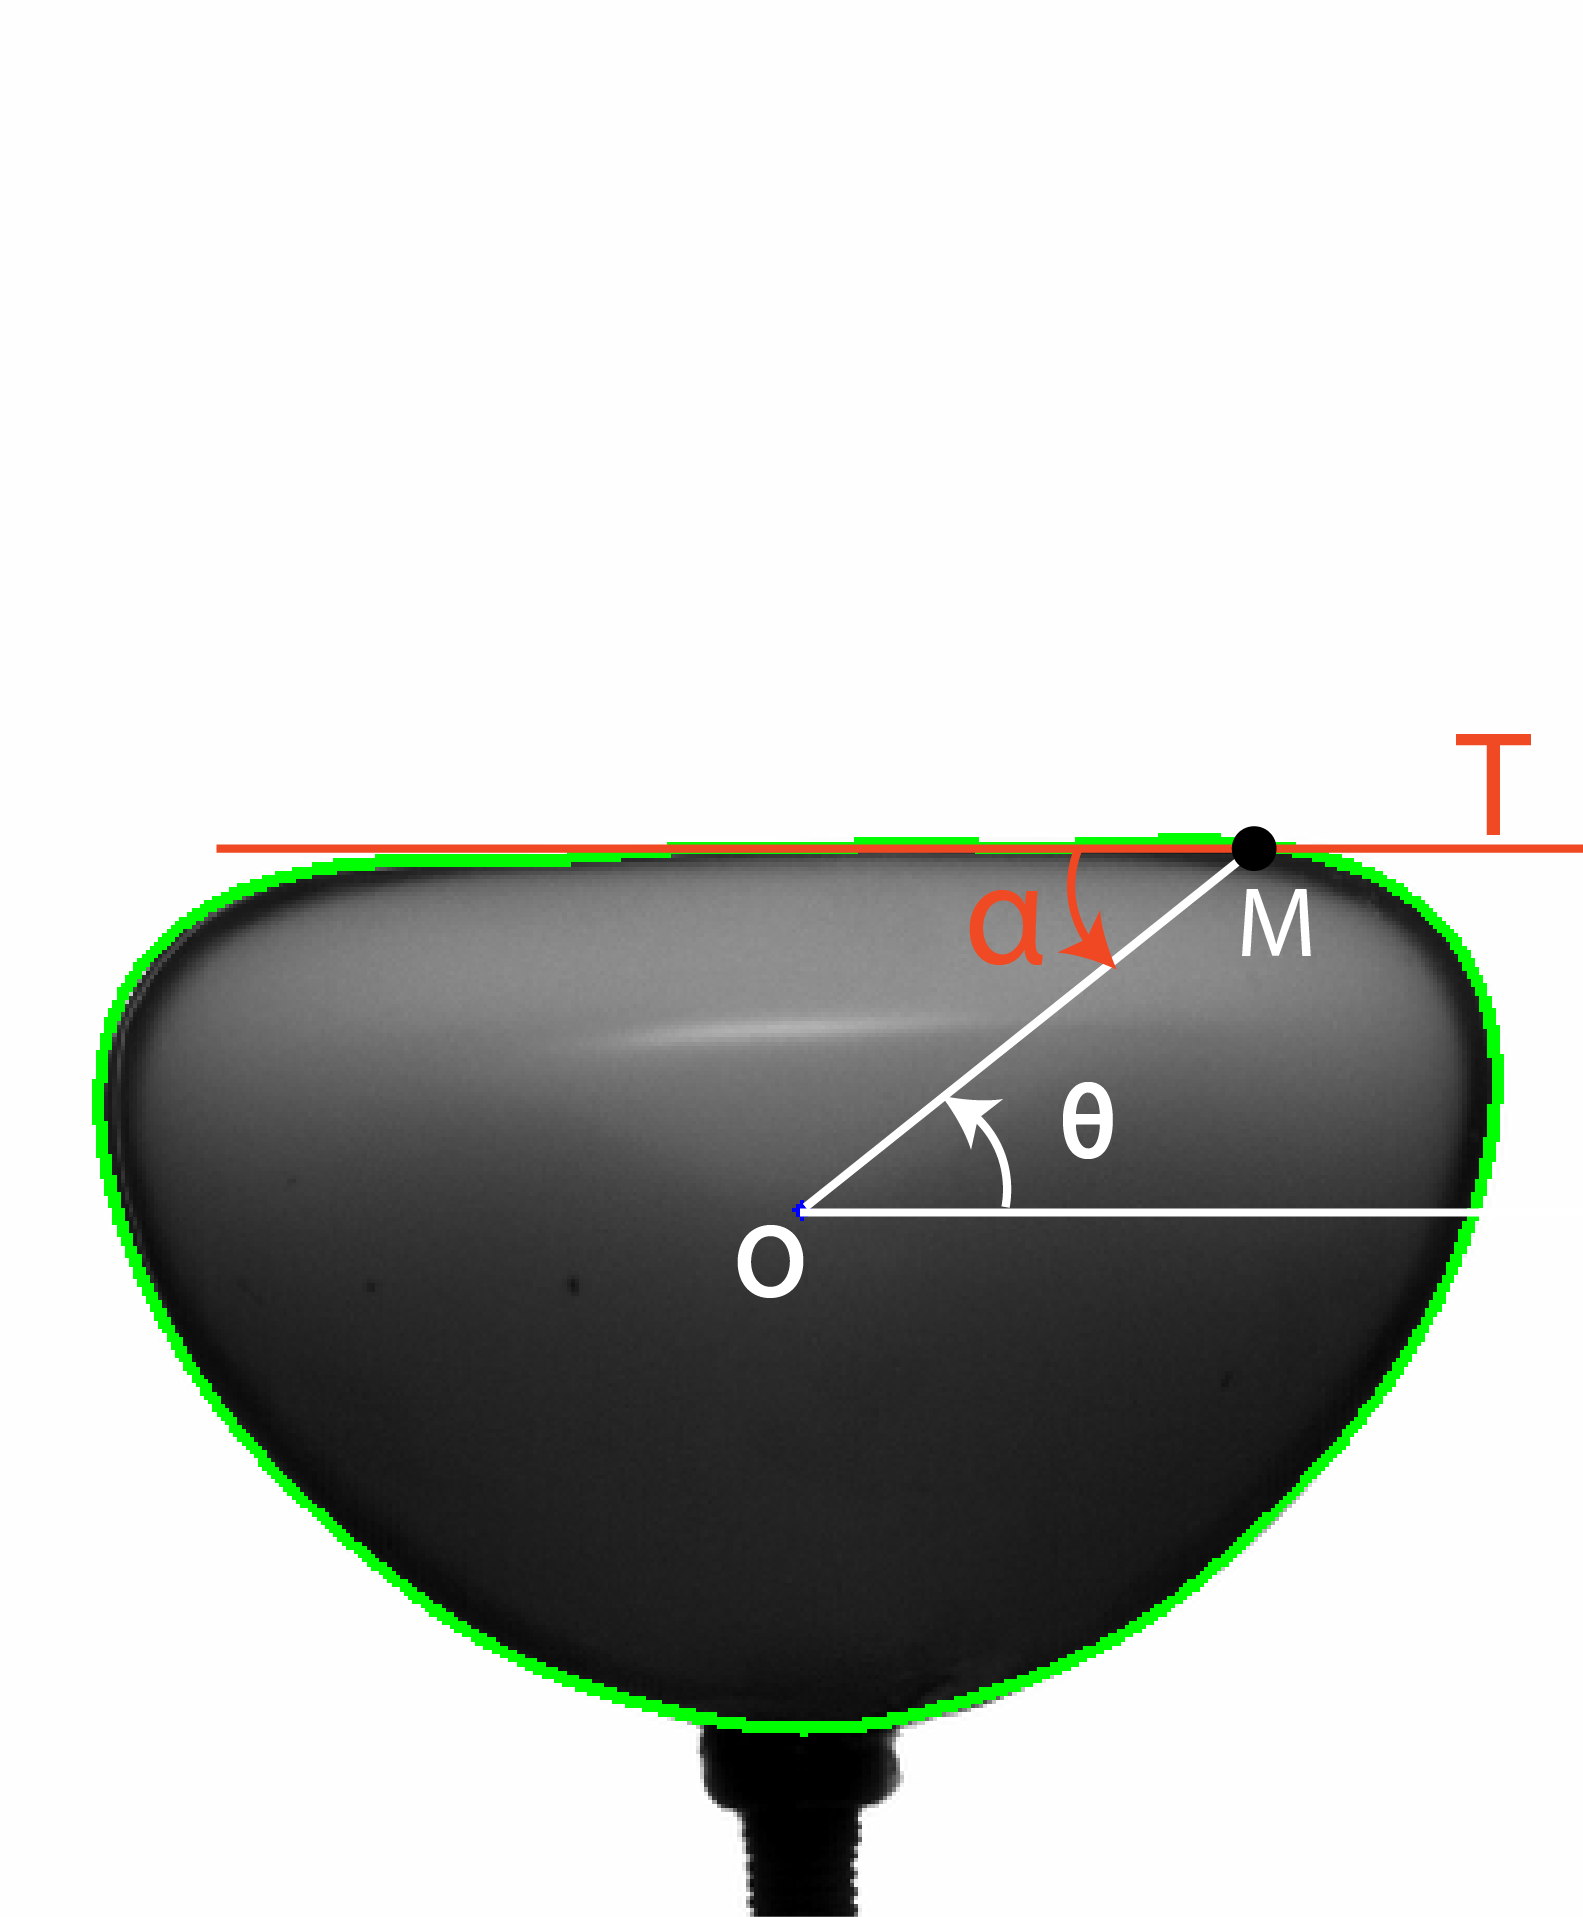
\includegraphics[width=0.48\textwidth]{figures/Chapter_1/tan_alpha.png}
	\caption{Definition of the horizontal tangent}
	\label{fig:Illustration_tangent}
\end{figure}
%Integrating \eqref{eq:tangent} in \eqref{eq:tangent_horizontal}, gives a condition on theta:
	%\begin{gather*}
		%\tan(\theta+\alpha) =0\\
		%\Rightarrow\frac{\tan(\theta)+\tan(\alpha)}{1-\tan(\theta)\tan(\alpha)} = 0\\
		%\Rightarrow\tan(\theta)+\tan(\alpha) = 0\\
		%\Rightarrow\tan(\theta)+|{\frac {\tilde{R}(\theta )}{\tilde{R}'(\theta )}}|=0\\
		%\Rightarrow\tan(\theta)+|{\frac {\sum\limits_{k=0}^M a_k \sin(\theta)^k  )}{\cos(\theta) \sum\limits_{k=1}^M k a_k \sin(\theta)^{(k-1)} )}}|=0
	%\end{gather*}
%The point $M(R_{h},\theta_h)$ is determined by minimizing this final expression.\\
The outer contour belonging to the shape generatrix is defined as:
\begin{equation*}
	\tilde{R}(\theta) = \sum\limits_{k=0}^M a_k \sin(\theta)^k
\end{equation*}
With $\theta \in[-\pi-\theta_h,\theta_h]$\\
The concavity experimental points with a polynomial which guaranties the continuity and differentiability at the $M(R_{h},\theta_h)$ point.
%Now, we need to fit the concavity experimental points with a functional which guaranties the continuity and differentiability at the $M(R_{h},\theta_h)$ point.\\
%To do so, we define a fitting functional as follows:
%\begin{align*}
%g(y) &= a x^6+b x^4+ c x^2+ d\\
%\intertext{with the following continuity conditions on $d$ and $c$}
%d &= -c x_{c}^2 - b x_{c}^4 -ax_{c}^6+ y_c\\
%\intertext{and}
%c &= -2 b x_{c}^2-3 a x_{c}^4
%\end{align*}
%Where $a,b,c,d$ are the fit parameters, and $x_c,y_c$ are the coordinates of the point $M(R_{h},\theta_h)$ in the cartesian coordiantes system, based around the center of the polar coordinate system, previously defined. Then, the extracted concavity experimental points are fitted with the 6-degree polynomial, using the $"`Levenberg-Marquardt"'$ method. \\
\paragraph{}
The combination of the two fits, determines an analytical description of the generatrix (fig.\ref{fig:fit_complet}), allowing the analytical calculus of the volume and the center of gravity of the capsule\footnote{The calculus of these two quantities being complex, is not developed here and can be found in the annexe.}. 
\paragraph{}
As precised earlier, the example treated here is the most complexe. In the case of a convex shape(non-buckled shape), only the outer contour fit is considered, and $\theta_h$ is equal to $\frac{\pi}{2}$.
\paragraph{}
The estimation of the error over the shape detection is set to the pixel level, and is around 0.1mm

%as follow:\\
%For the volume:
%\begin{align*}
	%V_{shape} &= V_{outer_contour}+V{concavity}\\
	%\intertext{Where:}
	%V_{outer_contour} & = \frac{2\pi}{3} \sum\limits_{i,j,k=0}^M a_i a_j a_k(\frac{1.-(\cos(\phi_h))^{(i+j+k)}}{(1.+i+j+k)})
	%\intertext{With:}
	%\phi_h &=\frac{\pi}{2}-\theta_h\\
	%\intertext{and: }
	%V{concavity} &= 2\pi((\sum\limits_{i=0}^3 \frac{1}{2(i+1)}x_c^{2(i+1)})-\frac{\tan(\phi_h)*x_c^3}{3})
%\end{align*}
%and for the gravity center:
%\begin{align*}
	%V_{shape} &= V_{outer_contour}+V{concavity}\\
	%\intertext{Where:}
	%V_{outer_contour} & = \frac{2\pi}{3} \sum\limits_{i,j,k=0}^M a_i a_j a_k(\frac{1.-(\cos(\phi_h))^{(i+j+k)}}{(1.+i+j+k)})
	%\intertext{With:}
	%\phi_h &=\frac{\pi}{2}-\theta_h\\
	%\intertext{and: }
	%V{concavity} &= 2\pi((\sum\limits_{i=0}^3 \frac{1}{2(i+1)}x_c^{2(i+1)})-\frac{\tan(\phi_h)*x_c^3}{3})
%\end{align*}

\begin{figure}[H] %
	\centering%
  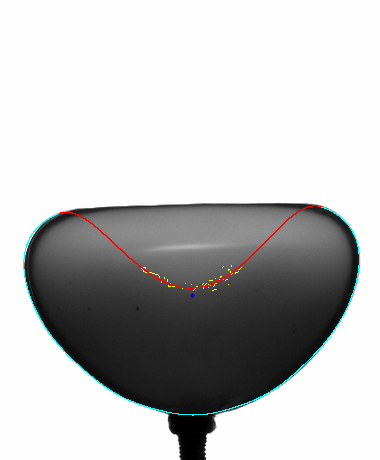
\includegraphics[width=0.48\textwidth]{figures/Chapter_1/outer_contour_complete.png}
	\caption{Fitted outer contour in blue, fitted concavity in red, and experimental concavity points in yellow}
	\label{fig:fit_complet}
\end{figure}
\newpage
\section{Frictionless rail}
\subsection{Brief introduction and motives}
\paragraph{}
The spring experiments allowed us to quantify the thrust induced by the buckling and unbuckling phases, in a situation where the shells are attached to a spring, but we wanted to go further by studying the shell dynamics and its interaction with the surrounding fluid in a configuration that allows more freedom. Keeping in mind that shells are light and float to the surface when left free of any attach, we needed to design an experimental setup which keeps the shell immersed and allows it to move freely at the same time.  One of the most elaborate attempt was to attach the shell to a support, itself fixed to a large plastic disc. The plastic disc/shell system is trapped between two non-miscible liquids\footnote{This condition comes from the fact that when pressurizing the tank, air is blown inside the tank creating a flow which may move the disc. To avoid this bias, a liquid is added on top of the disc, lighter than the system, allowing to damp the flow generated by the pressurization.} and managing to have large difference of density between them in order to increase the stability, while applying pressure externally. This setup would have allowed to study the 2-D motion of a spherical shell submitted to external pressure cycles, but unfortunately stability issues rose during the buckling and unbuckling phases which shift the center of gravity of the system and tilts the disc, preventing from having controlled and reproducible experiments.
\paragraph{}
To characterize the swimming, we kept the idea of a free swimmer but constrained the degrees of freedom to only one. The setup we used, consists in attaching a spherical capsule to a support, itself mounted on an frictionless air bearing, which can slide horizontally on a rail, allowing a 1-D translational displacement. The shell is immersed in a liquid, as represented in figure \ref{fig:experimental_setup_frictionless_rail}. Contrary to the spring experiment where the shell deformation is actuated by applying a positive relative pressure inside a tank, in the Frictionless rail experiment, this option was not chosen, due to the complexity of the experimental setup it would have required: Building a bigger tank designed to host a $600$ mm long rail, and apply two different pressure ranges, one to supply the truck with a 5-6 bar pressure, and another range between 0 and 2 bar applied inside the tank. Instead, the shape deformation cycles are actuated by applying negative pressure cycles to the air volume enclosed in the spherical capsule. This is done by connecting the enclosed volume to a pressure controller, through a flexible pipe. In order to have a better control over the experimentation, a weakness is introduced, by reducing the thickness locally by 0.2 mm, which allows to define where the instability will occur. The buckling spot is oriented in a direction parallel to the rail, to ensure the capture of the full displacement during the buckling and unbuckling phase. The position of the support and the shell deformation are captured using a high-speed camera. 
%Several control parameters were explored:
%\begin{itemize}
	%\item The thickness of the capsule's shell, to vary the elastic energy stored by it.
	%\item The dissipation property of the material in which the spherical capsules are cast.
	%\item The viscosity of the swimming medium.
	%\item And, the proximity to a wall.
%\end{itemize}
%The advantage of this experiment is that it allows to directly illustrate the swimming, to quantify it and to measure the thrust during the buckling and unbuckling phase.
\begin{figure}[H] %
	\centering%
	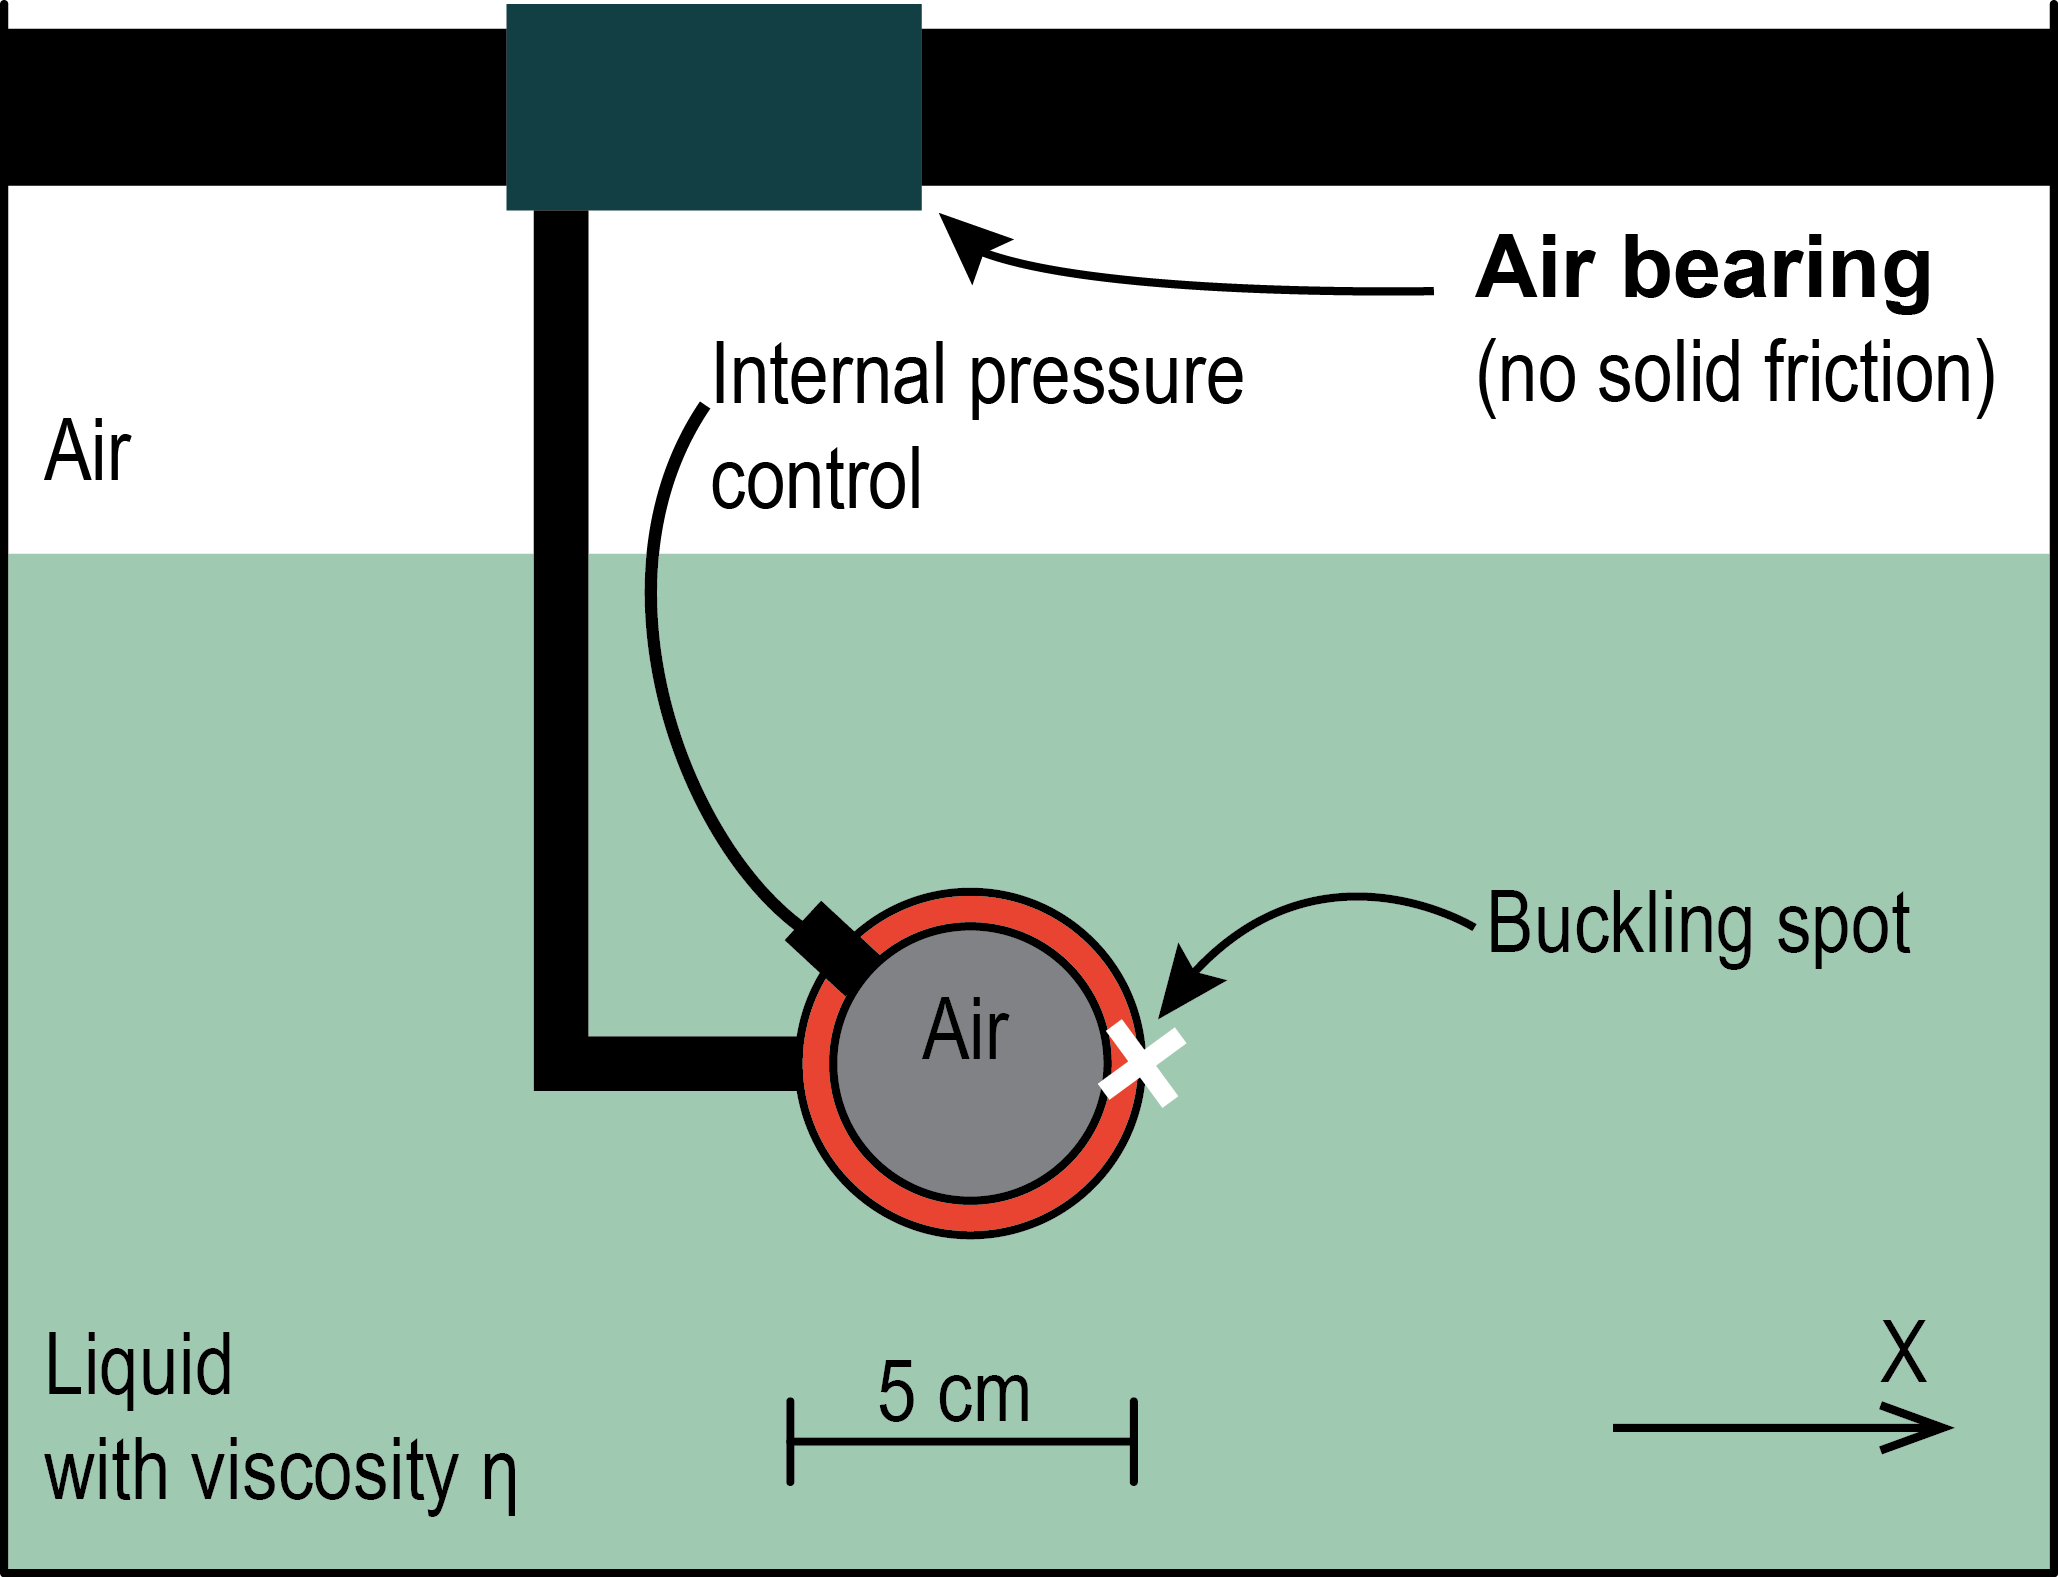
\includegraphics[width=\textwidth]{figures/Chapter_1/schematic_experimental_setup_fr.png}
	\caption{Schematic representation of the frictionless rail experimental setup}
	\label{fig:experimental_setup_frictionless_rail}
\end{figure}
\subsection{Equipment}
\subsubsection{Air bearing system}
\paragraph{}
The air bearing rail system manufactured by "`Air Way \texttrademark"' (fig.\ref{fig:pic_frictionless}), is composed of two main components made of black anodized aluminum. The first component is a 600mm long and 75mm large T-shaped rail, which serves as a guide to the second component, being the truck. The truck is designed to slide along the guide without solid friction. This is possible thanks to microscopic holes present in the inner surface of the truck. These holes allow pressurized air to stream on the surface of the guide and create a cushion air, which prevents the surfaces of the guide and the truck from being in contact. The air pressure which is provided to the truck through its inlet, sets the load capacity.
\begin{figure}[H] %
	\centering%
	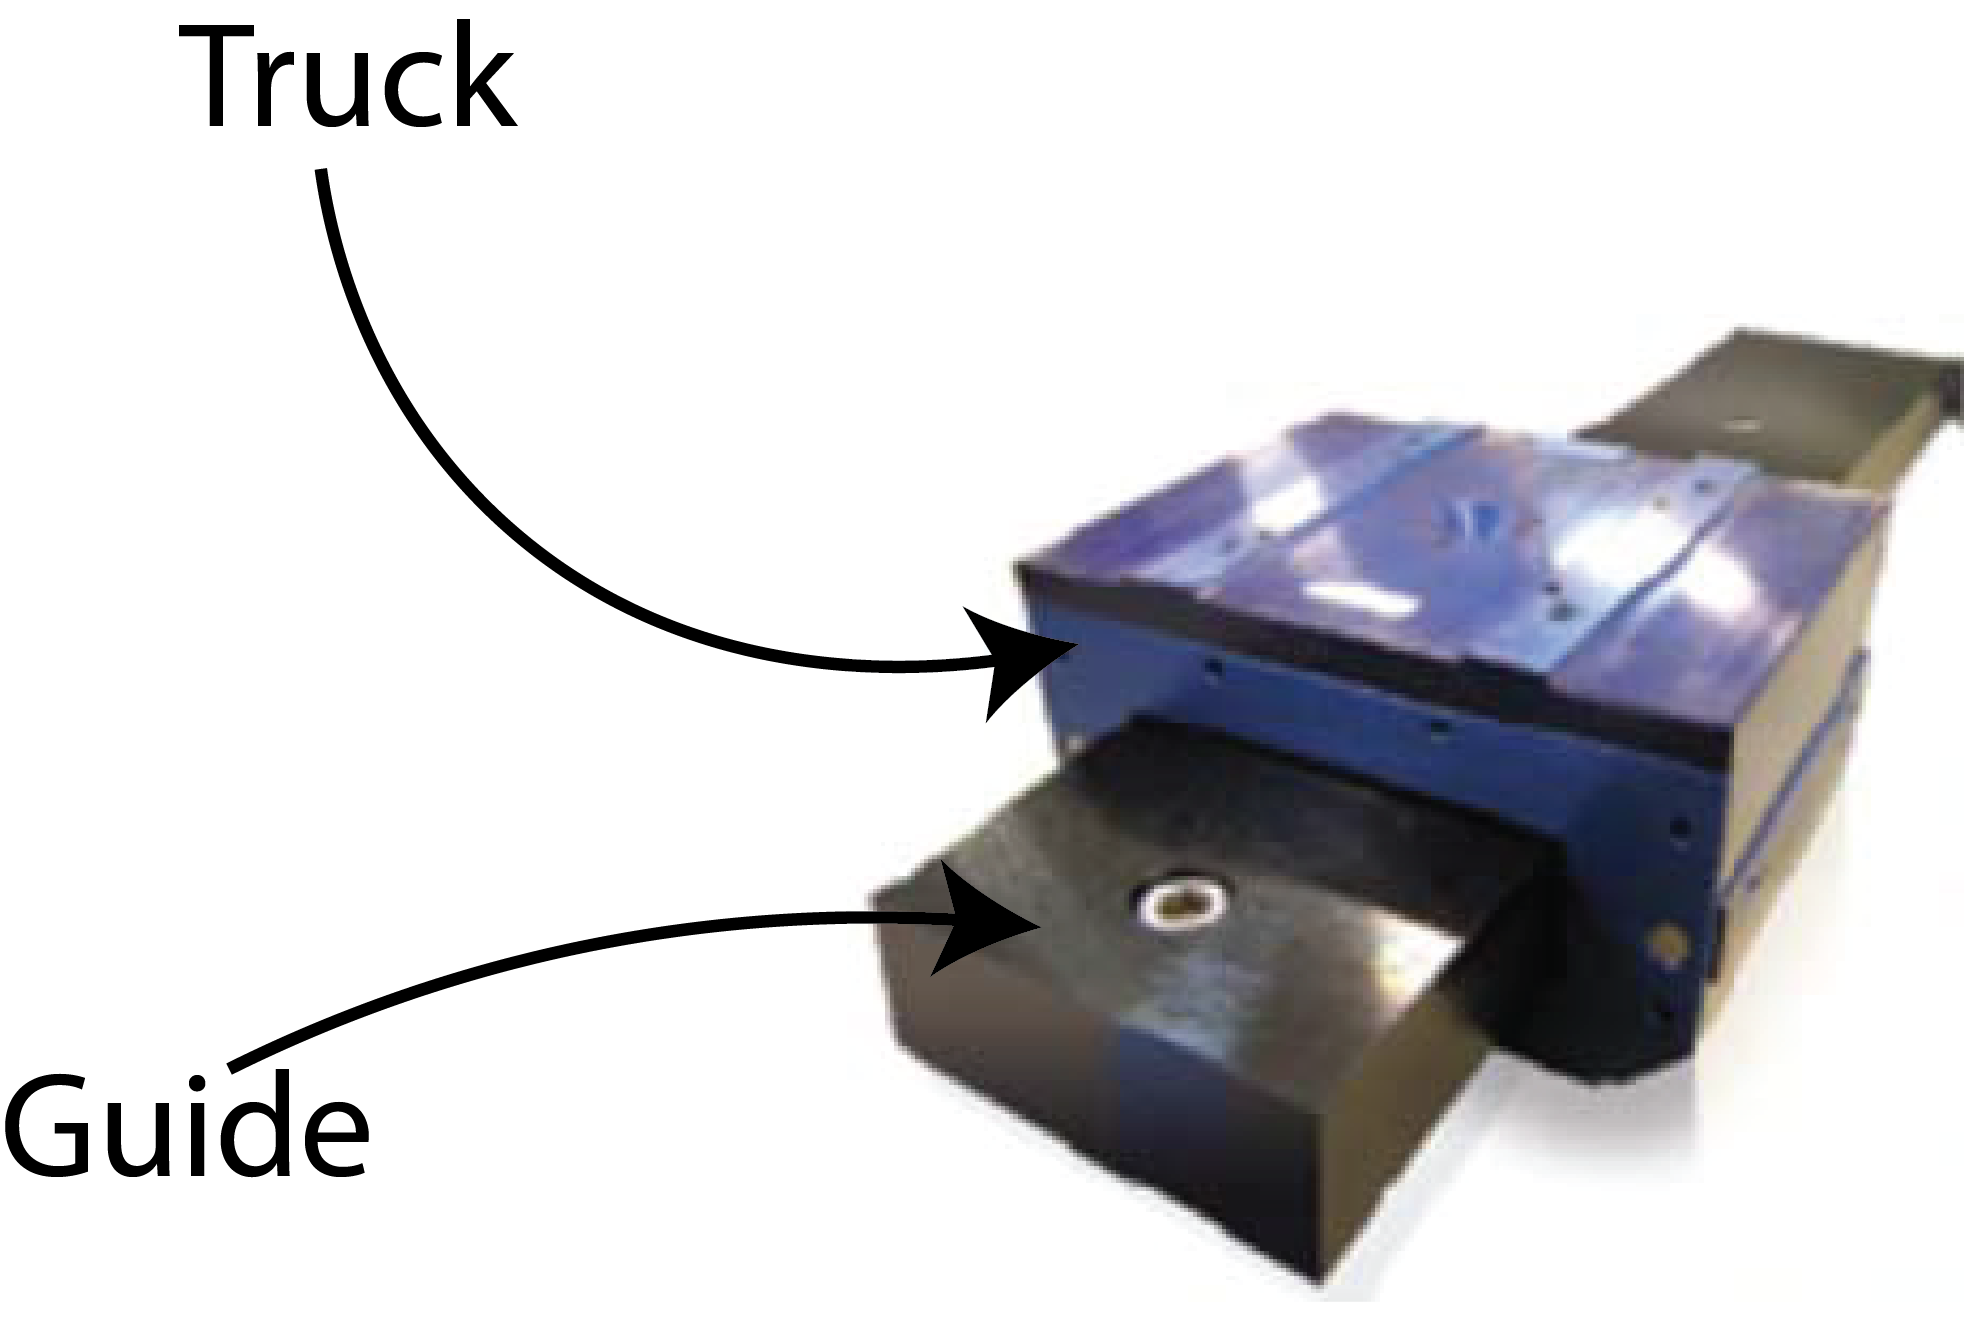
\includegraphics[width=0.48\textwidth]{figures/Chapter_1/Airbearing.png}
	\caption{Illustration of the air bearing system}
	\label{fig:pic_frictionless}
\end{figure}
In the case of the experiment, the input pressure was of 5 bars. This pressure allows the loads precised in \ref{tab:pressure_truck}. These maximum loads are big compared to the forces involved in the experiment. For example, the max buoyancy force plus the weight of the truck give a total of 11N.\\
A flexible tube is used to link the air pressure source to the truck pressure input. The tube is suspended at a 2m height and left loose, to avoid any bending or tension force which might displace the truck and lead to a measurement error.
\begin{table}[H]
	\centering
		\begin{adjustbox}{width=\textwidth}
			\begin{tabular}{|c|c|c|c|}
				\hline
				Input pressure (bar) & horizontal load (N)&Vertical load (N)& maximum moment force in the three directions (Nm) \\
				\hline
				6&473&709&2.8\\
				\hline
			\end{tabular}
		\end{adjustbox}
	\caption{Load capacity for a 5 bar pressure}
	\label{tab:pressure_truck}
\end{table}
\paragraph{}
The rail is mounted on two slides, which can translate vertically on two rigid extruded aluminum profiles(fig.\ref{fig:setup_rail}). This allows to set the rail at the horizontal plane, using an electronic spirit level. This operation is necessary, to ensure that no drift is produced, which may lead to unsatisfactory measuring precision.
\begin{figure}[H] %
	\centering%
	\includegraphics[width=0.48\textwidth]{figures/Chapter_1/setup_rail.pdf}
	\caption{Picture representing the experimental setup to mount the rail}
	\label{fig:setup_rail}
\end{figure}

\paragraph{}
All technical details associated to the air bearing system can be found in the appendix \ref{Appendix A}.
\subsubsection{Mounting support}
\paragraph{}
To link the spherical shell to the truck, a L-shaped mounting support was realized made of Aluminum (fig.\ref{fig:mounting_support}. This support is supplied with a tapped hole to fix it to the truck and a tapped hole to connect it to the spherical shell, through a suction cup. The support weighs 220g, in addition to the 1300 g of the truck. Other materials and designs were considered to make a lighter support, but we found out that the thrust produced during the buckling phase, was able to bend the support, which alters the displacement produced and introduces a bias in the experiment and its physical interpretation.
\begin{figure}[H] %
	\centering%
	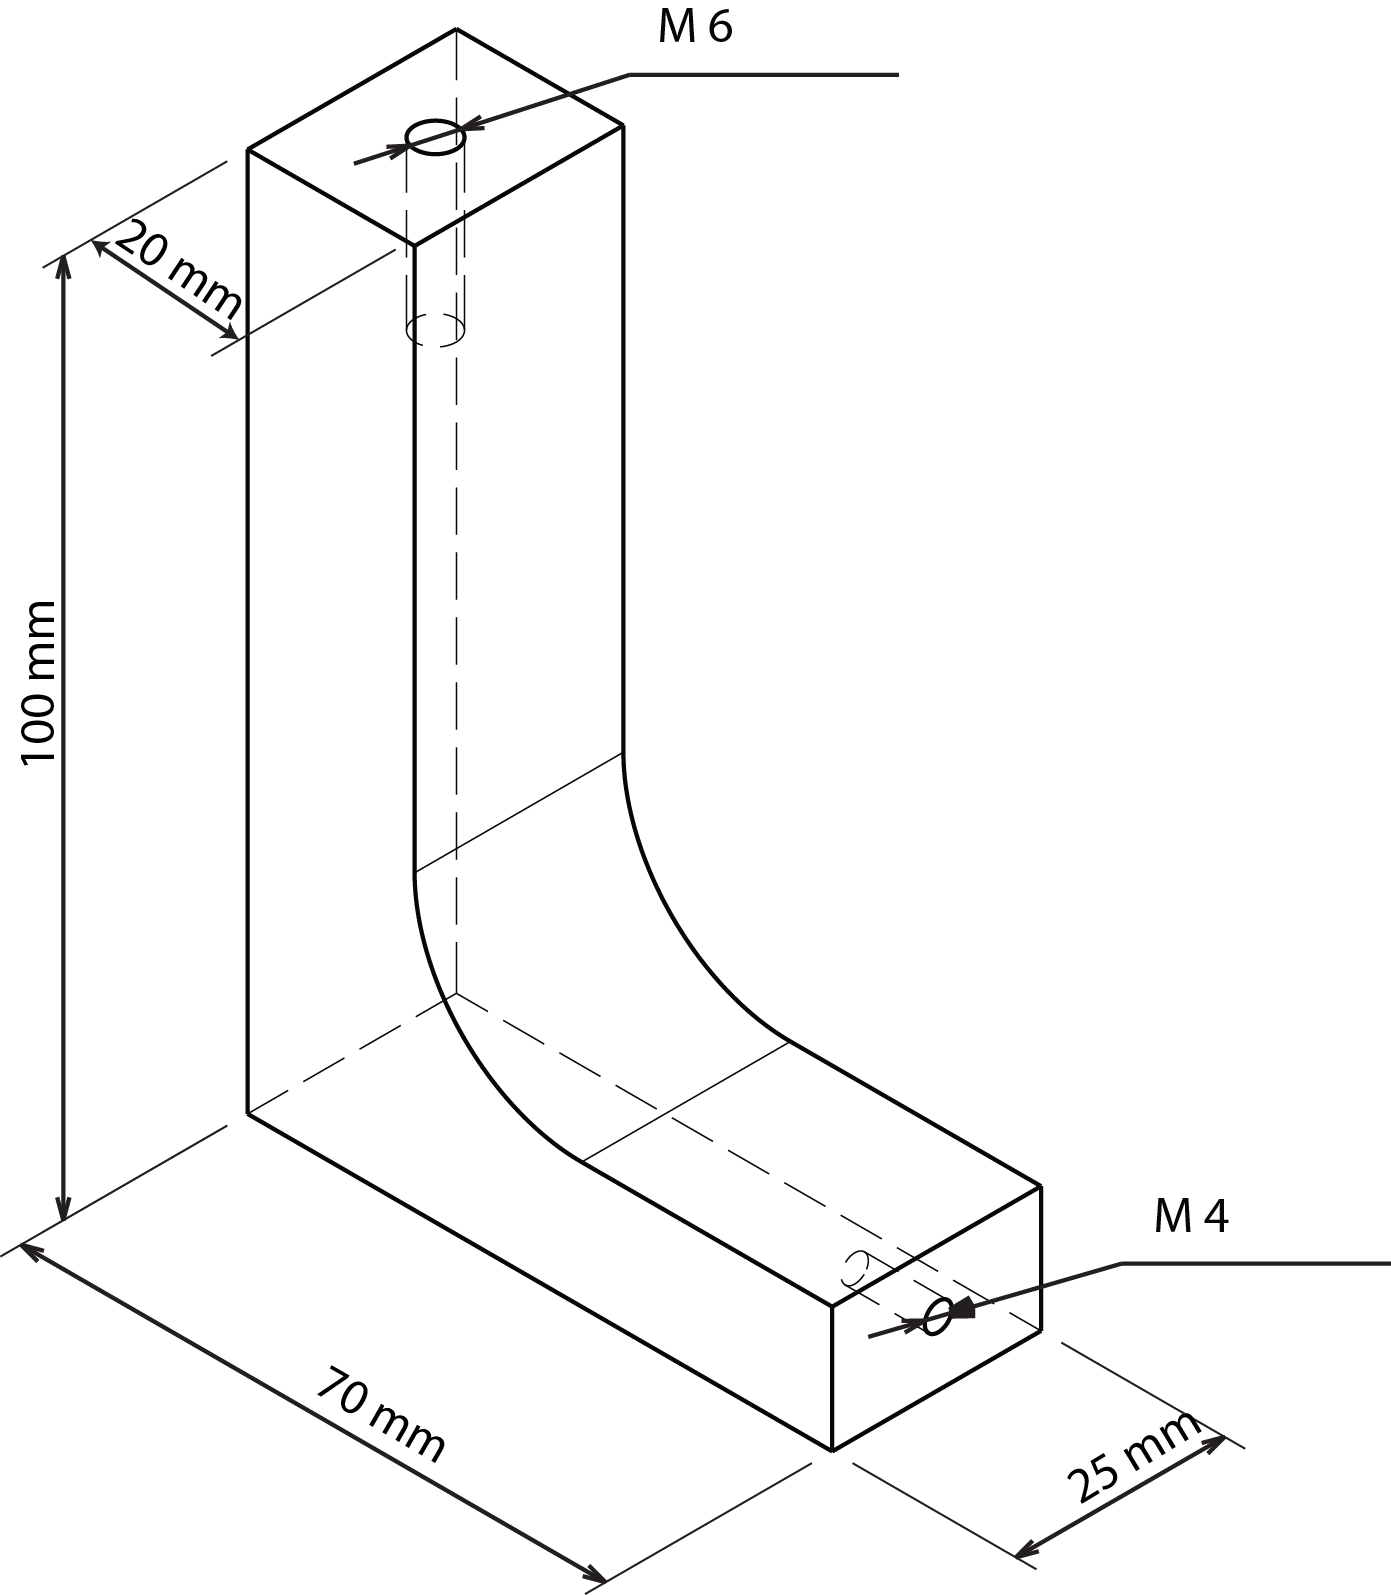
\includegraphics[width=0.48\textwidth]{figures/Chapter_1/Support.png}
	\caption{Schematics of the mounting support}
	\label{fig:mounting_support}
\end{figure}


\subsubsection{Pressure controller}
\paragraph{}
The pressure controller used in this experiment has been presented earlier in the spring experiment (\ref{sssection:pressure_controller}). This time, it is operated on the [-1,1] bar channel and required the use of a vacuum pump to reach -1 bar.
\subsubsection{Tank}
\paragraph{}
The tank used in this experiment, is an open recipient, with 340mm by 170mm rectangular base and 250 mm height, made out of glass.  
\subsubsection{Camera,lenses and light sources}
The equipment used for the experiment is the same as in the spring experiment (\ref{sssection:CLLS}). In addition, a macro lens with a fixed focal length $f= 100$ mm with a maximum aperture of f/2.0 was used to zoom over a region of interest, without losing in spatial resolution.
  
\subsection{Experimental process}
\paragraph{}
%This experimental setup has a rich potential, allowing the exploration of a multitude of physical quantities, and different configurations can be imagined to enrich it even more. We tried however, to focus our experimental investigations on the effect of primary physical quantities over the swimming. The quantities explored are:
Experimental investigations were focused on the effect of primary physical quantities over the swimming. The quantities explored are:
\begin{enumerate}
	\item The effect of the amount of elastic energy stored prior to buckling on the swimming efficiency. This is done by varying the thickness of the shell, keeping the outer radius constant, and this is performed with the set of three shells cast out of "`Drangon skin"'\textregistered material.
	\item The effect of solid dissipation on the swimming efficiency, by varying the rebound resilience of the material in which the shell is cast. This quantity refers to the restitution rate of the stored elastic energy. To isolate its effect, two materials were chosen with the specificity of sharing the same elastic modulus, and two shells with an identical thickness were cast.
	\item When at proximity to a wall, with the buckling spot facing it, the swimming induced by the buckling and unbuckling phases is modified. To study this effect, two series of experiments are conducted, one far from the wall, to characterize the swimming in bulk, and the second one near the wall to study the effect of directional confinement.\footnote{Only the frontal wall proximity is investigated, the lateral, rear or any other angular configurations are to be studied in the future}. 
\end{enumerate}
\paragraph{}
All the enumerated experiments above, are conducted for different viscosities of the swimming medium, to vary the $Re$ number characterizing the flow regime. To do so, seven "`water-glycerol"' solutions were prepared, with viscosities ranging from 0.001 Pa.s with (100\% Water-0\% glycerol) solution  to 1.3 Pa.s with a (0\% Water-100\% glycerol) solution, with a targeted viscosity step of half a decade, taking advantage of the miscibility of the (water-glycerol) couple. To target the desired viscosity, the volume fraction of each liquid needs to be calculated precisely, because the viscosity of a water-glycerol solution evolves in a non-linear way\cite{viscositynonlinearCheng}. To approach the targeted viscosity, the volume fractions were calculated using an empirical formula found in the literature\cite{viscositynonlinearCheng}. A sample is collected at the end of the experiment and its viscosity is measured at the experiment temperature range.\\
In addition, experiments are conducted in a liquid called "`UCON Lubricant 75-H-90,000 "`, which has a viscosity of 37 Pa.s at room temperature, providing another decade to the viscosity range explored. All the water-glycerol solutions are transparent, and the "`UCON Lubricant"' presents a yellowish coloration which does not prevent the visualization during the experiment. 
Table\ref{tab:viscosities} summarizes the solutions in which the experiments are conducted.
\begin{table}[H]
	\centering
		\begin{adjustbox}{width=\textwidth}
			\begin{tabular}{|c|c|c|c|}
				\hline
				Solution number & liquid volume fractions & targeted viscosity at 20°C (Pa.s)\\
				\hline
				1&100\% Water-0\% glycerol&0.001\\
				2&59\% Water-41\% glycerol&0.005\\
				3&47\% Water-53\% glycerol&0.01\\
				4&26\% Water-74\% glycerol&0.05\\
				5&19\% Water-81\% glycerol&0.1\\
				6&6.4\% Water-93.6\% glycerol&0.5\\
				7&0\% Water-100\% glycerol&0.5\\
				8&100\% Ucon oil&37\\
				\hline
			\end{tabular}
		\end{adjustbox}
	\caption{Summary of the solutions prepared.}
	\label{tab:viscosities}
\end{table}
  
\subsubsection{Experimental protocol}
\paragraph{}
Once the volume fractions for a targeted viscosity are calculated, a 20L solution is prepared, and an experimental protocol is followed for each one of the 5 capsules to be studied:
\paragraph{Preliminary settings}
First, the spherical shell is connected to the mounting support via a suction cup that is, on one hand, glued to the spherical shell and on the other hand screwed to the M4 tapped hole in the mounting hole.\\
The system "`support-capsule"' is immersed at the liquid's mid height. This step is followed by a horizontality check of the fictionless rail, using a spirit level, allowing a 0.001 rad precision.\\
Then, rail pressure inlet is supplied with a 5 bar air pressure, and the truck is positioned at the middle of the 340 mm long tank.\\
\paragraph{Multiple pressure cycles}
To study the displacement produced by the shape deformation, 20 successive pressure cycles of a period of 15s, are applied to the volume enclosed in the spherical shell, and images of the "`support-capsule"' system are recorded at 24 FPS (fig.\ref{fig:illustration_frictionless_rail}).The pressure cycles applied begin by  a 5s descending pressure ramp until reaching the buckling critical $\Delta P$, followed by a plateau at a the same pressure for 2.5s. The pressure is increased through a 6.5s ascending pressure ramp, until reaching the unbuckling $\Delta P$\footnote{The unbuckling $\Delta P$ can be positive sometimes for small thicknesses, due to the fact that the shell collapses completely on itself and obstructs the hole which communicates with the pressure controller. To force the shape to unfold, pressurized air is injected inside the capsule inner volume.} and is followed by a 1s plateau (fig.\ref{fig:pressure_cycle_fr}.\\
Temperature measurement are performed at the beginning and at the end of the pressure cycles.
\begin{figure}[H]%
	\centering%
	 \begin{subfigure}[h]{0.48\textwidth}%
        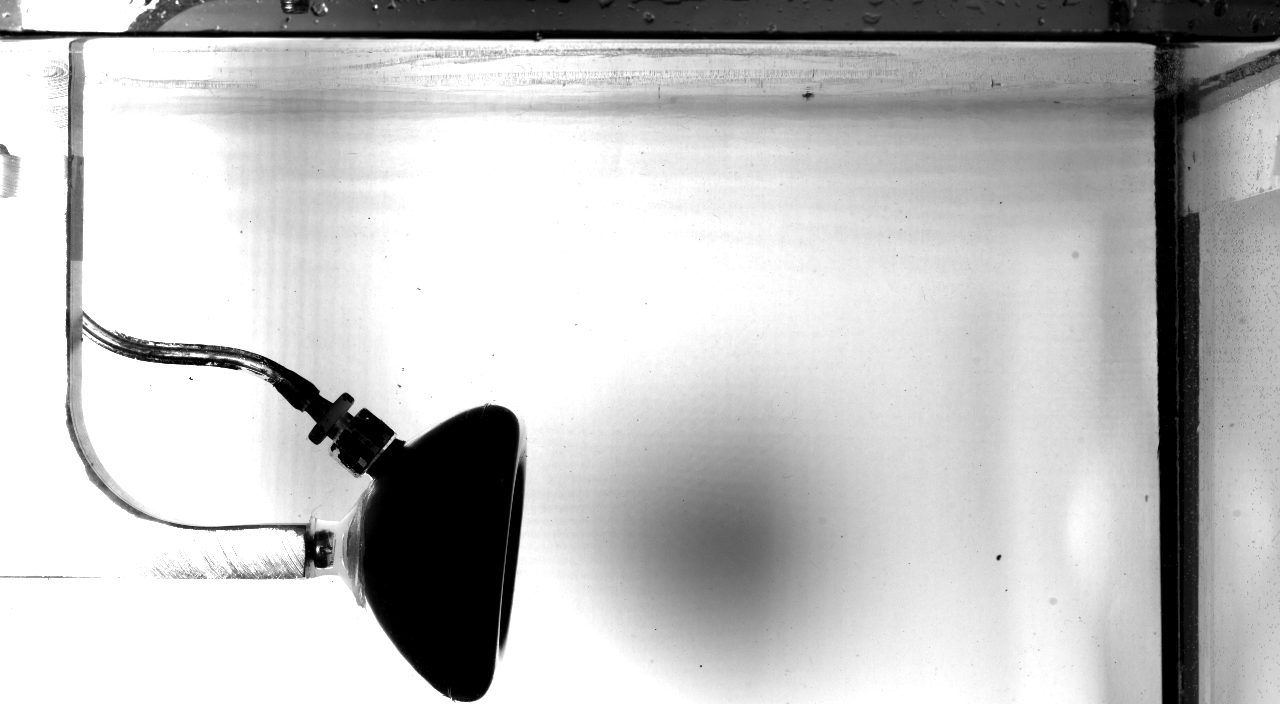
\includegraphics[width=\linewidth]{figures/Chapter_1/cycles_lp_00241.png}%
        \caption{Deflated state}%
    \end{subfigure}%
    \begin{subfigure}[h]{0.48\textwidth}%
        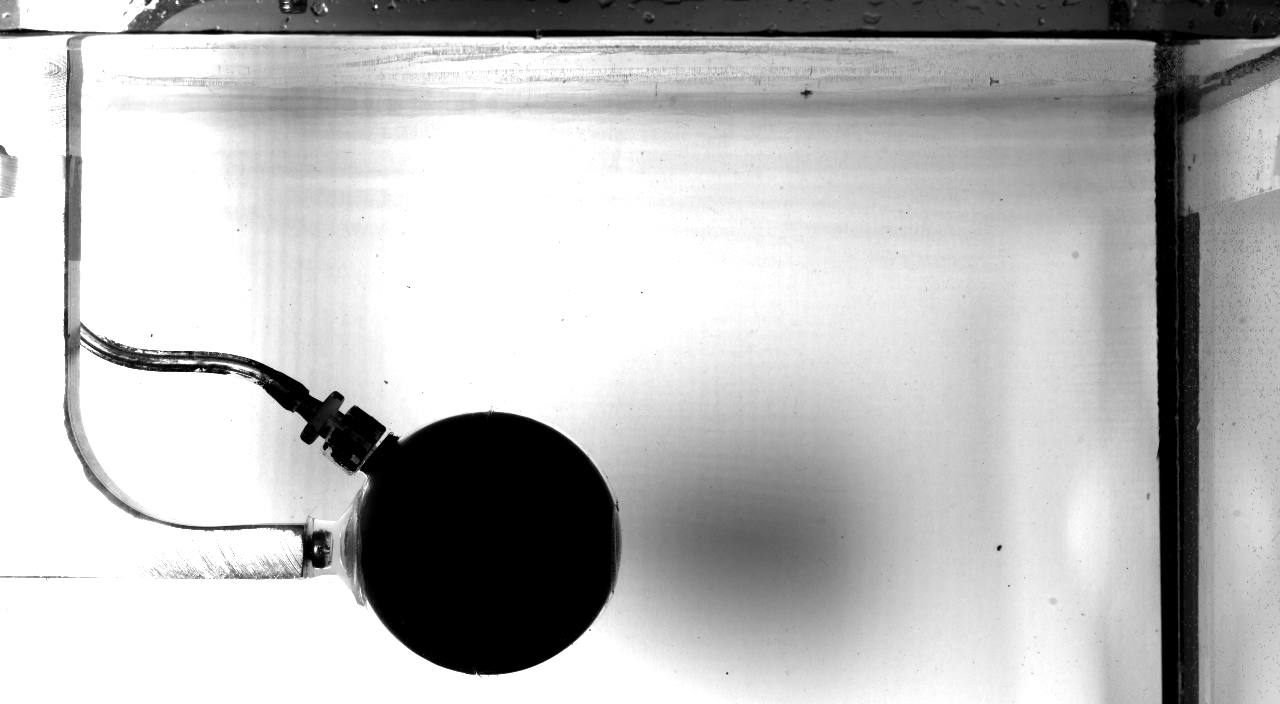
\includegraphics[width=\linewidth]{figures/Chapter_1/cycles_lp_00001.png}%
        \caption{Inflated state}%
    \end{subfigure}%
		\caption{Illustration of the recorded images during the two plateaux of the pressure cycle}
		\label{fig:illustration_frictionless_rail}
\end{figure}
 \begin{figure}[H]%
	\centering%
	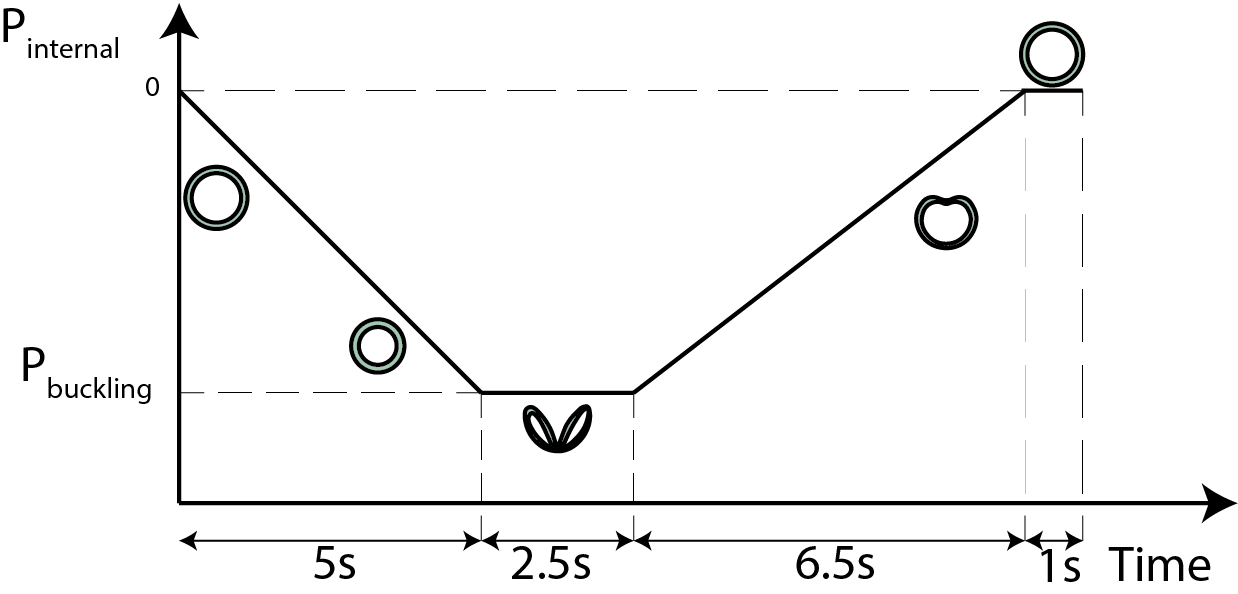
\includegraphics[width=\textwidth]{figures/Chapter_1/pressure_cycle_fr.png}
	\caption{Qualitative representation of the pressure cycles}
	\label{fig:pressure_cycle_fr}
\end{figure}

\paragraph{}
To study the displacement produced by the shape deformation near a wall, the "`support-capsule"' is brought at a distance where the tip of the spherical shell is at 25mm from the wall and the same process stated previously is followed.
 %20 successive pressure cycles of a period of 15s, are applied to the volume enclosed in the spherical shell, and images of the "`support-capsule"' system are recorded at 24 FPS (fig.\ref{fig:illustration_frictionless_rail_wall}).\\
%Temperature measurement are performed at the beginning and at the end of the pressure cycles.
%\begin{figure}[H]%
	%\centering%
	 %\begin{subfigure}[h]{0.48\textwidth}%
        %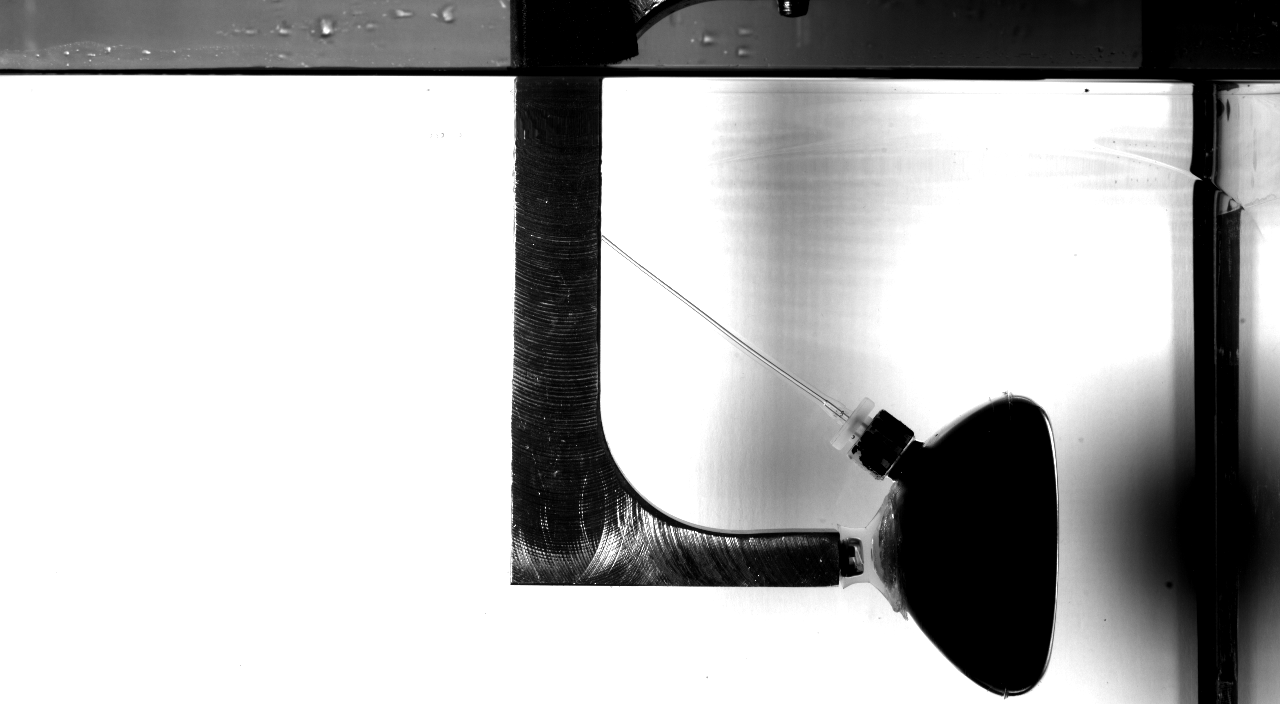
\includegraphics[width=\linewidth]{figures/Chapter_1/cycles_pp_00220.png}%
        %\caption{Deflated state}%
    %\end{subfigure}%
    %\begin{subfigure}[h]{0.48\textwidth}%
        %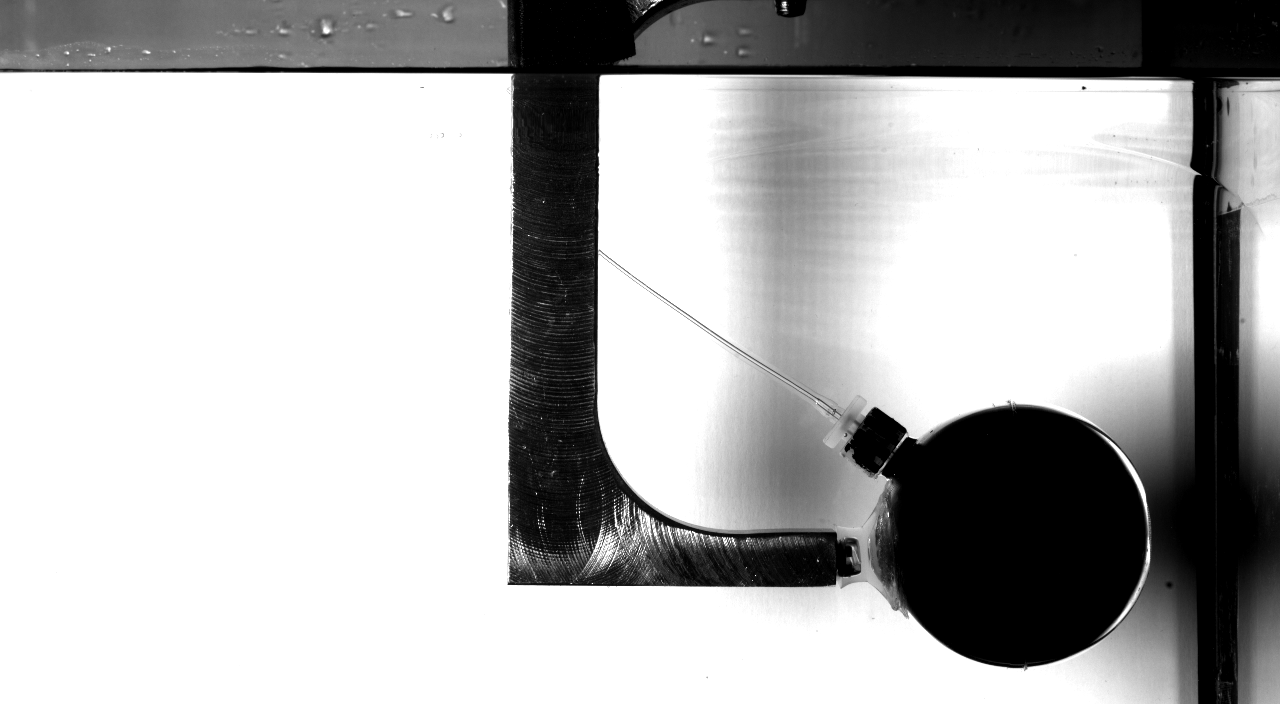
\includegraphics[width=\linewidth]{figures/Chapter_1/cycles_pp_00001.png}%
        %\caption{Inflated state}%
    %\end{subfigure}%
		%\caption{Illustration of the recorded images during the two plateaux of the pressure cycle, near a wall}
		%\label{fig:illustration_frictionless_rail_wall}
%\end{figure}
%\paragraph{}
%The spherical shell is brought in contact with the wall and a reference image is recorded. This configuration will be defined as the zero in the position axis, and all the distances measured will be done relatively to this configuration.
\paragraph{High temporal resolution recordings}
In order to quantify the shape deformation cycle, a high temporal resolution is needed. To do so, the truck is positioned at the middle of the tank, a pressure cycle is applied (with the same settings as in the previous step), and images are recorded at 600FPS. This operation is iterated three times to have an estimation of the error. \\
Temperature measurement are performed at the beginning and at the end of the each iteration.
\paragraph{Drag-coefficient measurements}
In order to extract the thrust produced during the buckling and unbuckling phases, it is necessary to measure the drag force, independently. To do so, the truck is brought to the middle of the tank and is given an initial velocity. Images are recorded at 600 FPS. This is done in two constant deformation configurations: a spherical shape configuration to account for the drag coefficient when the shell is unbuckled, and a collapsed concave configuration to account for the drag coefficient when the shell is buckled.\\
Temperature measurement are performed at the beginning and at the end of the each iteration.
\paragraph{}
Table\ref{tab:pressure_cycle_configuration} summarizes the pressure cycle settings for all the studied spherical shells.
\begin{table}[H]
	\centering
		\begin{adjustbox}{width=\textwidth}
			\begin{tabular}{|c|c|c|c|c|}
				\hline
				Capsules & Buckling pressure (mbar) & Unbuckling pressure (mbar)&period (s)\\
				\hline
				$\frac{d}{R} = 0.08 $ & -100& 100 & 15\\
				$\frac{d}{R} = 0.22 $ & -600& 0 & 15\\
				$\frac{d}{R} = 0.30 $ & -1000 &  0 & 15\\
				\hline
				"`AJO 121"'& -200 & 100 & 15\\
				"`AJO 122"'& -350 & 100 & 15\\
				\hline
			\end{tabular}
		\end{adjustbox}
	\caption{Experimental pressure cycle parameters for the frictionless rail experiment}
	\label{tab:pressure_cycle_configuration}
\end{table}
\subsection{Image treatment}
\paragraph{}
The image treatment needed for the frictionless rail is relatively lighter compared to the one needed for the spring experiment, because the gravity center was of the shell was impossible to extract. It can be summarized as follows:
\begin{enumerate}
		
	\item From the multiple cycles set of experiments, the successive position of the system, after buckling and unbuckling phases are retrieved, by detecting the edge of the support, using the Canny edge detector algorithm.
	
	\item From the high-resolution set of experiments, the temporal evolution of the height of the convex envelop $H(t)$ (see fig.\ref{fig:h_t}) is retrieved, using the Canny edge detector algorithm.
	\begin{figure}[H] %
	\centering%
	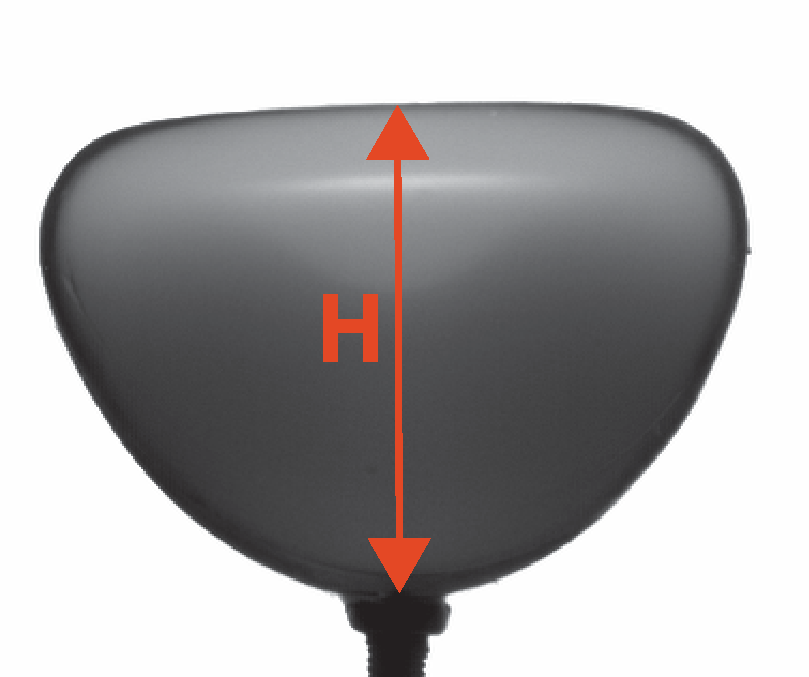
\includegraphics[width=0.48\textwidth]{figures/Chapter_1/h.pdf}
	\caption{Illustration of the height of the convex envelop}
	\label{fig:h_t}
\end{figure}
	\item From the drag-coefficient measurements set of experiments, the position of the support is tracked through time.
\end{enumerate}
\paragraph{}
%The displacements measured in this experiment, does not correspond exactly to the displacement of the system's center of gravity. This is due to the fact that, using this setup, it was not possible to track the shell's center of gravity. Knowing that, the only part of the system that gets deformed is the shell, and that it weighs more than 50 times less than the "`support/truck"' rigid sub-system, we can safely say that any shift of the system's center of gravity due to the deformation is small and within the margin of error.To quantify it, we use this formula:
 %****Put the formula of center of gravity as function of d/R****
%***   
Overall, the estimation of the error over the position detection is set to the pixel level, and is around 0.19mm. The net displacement per cycle is measured by taking the initial position of the support and the position of the support at the end of the 20 cycles, divided by the number of cycles. In this case, the error is set to 0.0095mm. The measurement of the displacement induced by the buckling and the displacement induced by the unbuckling , corresponds to the mean value of these displacements over 20 cycles, and the error is set to the standard deviation of the measurement sample.

\section{Particle-image velocimetry measurements}
\subsection{Brief introduction and motives}
\paragraph{}
To understand the evolution of the displacement obtained in the deflating and the re-inflating of the spherical shell, and how it is affected by the viscosity of the surrounding medium, it was necessary to understand the flow generated during both phases and how this flow changes with the fluid viscosity.
\paragraph{}
To do so, particle-image-velocimetry measurements (PIV) were performed in two distinct viscosities: water and glycerol.
\paragraph{}
particle-image-velocimetry measurement method is a non-intrusive method which simultaneously provides the instantaneous spatial flow field description and a quantitative result. its principle is based on the measurement of the displacement of small tracer particles that are carried by the fluid during a short time interval. The tracer particles used need to be sufficiently small and neutrally buoyant in order to accurately follow the fluid motion and not alter the fluid properties or flow characteristics. The tracer particles are illuminated by means of a thin light sheet generated from a source light and the light scattered by them is recorded onto two successive image frames by a high-speed camera. The recorded images are processed offline on a computer to extract the Eulerian velocity field. Figure \ref{fig:piv_principle} schematically describes the principle of the PIV measurement.
\begin{figure}[H]%
	\centering%
	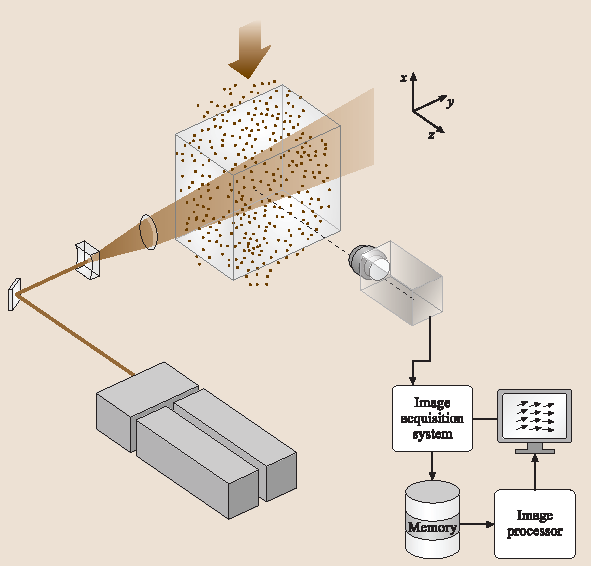
\includegraphics[width=\textwidth]{figures/Chapter_1/PIV_principle.pdf}
	\caption{Principle of Particle Image Velocimetry}
	\label{fig:piv_principle}
\end{figure}
\paragraph{}
The experimental setup (fig.\ref{fig:piv_schematics}) used to investigate the flow produced during the buckling and unbuckling phases consists of attaching the. 
spherical shell to a fixed support, orienting buckling spot vertically. The system was immersed in a glass tank of 50x50x50 cm tank, filled by either water or glycerol, previously seeded with $10$-$30$ $\mu$m  particles. A 1 mm vertical thin light sheet was produced using A continuous laser source runs through an tunable optical system. Just like the frictionless rail experiment, pressure cycles were applied to the air volume enclosed in the spherical shell by connecting it to the pressure controller through a flexible tube. A high-speed camera was carefully aligned in the direction normal to the light-sheet plane\footnote{Only one high-speed camera was needed because we assumed that the flow is axis-symmetric and negligible out-of-plane velocity component, two velocity components are enough to characterize the flow. If out-of-plane velocity component is not negligible, stereo-PIV measurement need to be performed using two cameras with an angle $\neq 90$\degree, in order to have the 3 velocity components.}.\\ The experiments were conducted in collaboration with "`Henda Djeridi"' at the "`LEGI"' laboratory who have a solid experience in PIV measurements and the adequate equipment to realize it.
\begin{figure}[H]%
	\centering%
	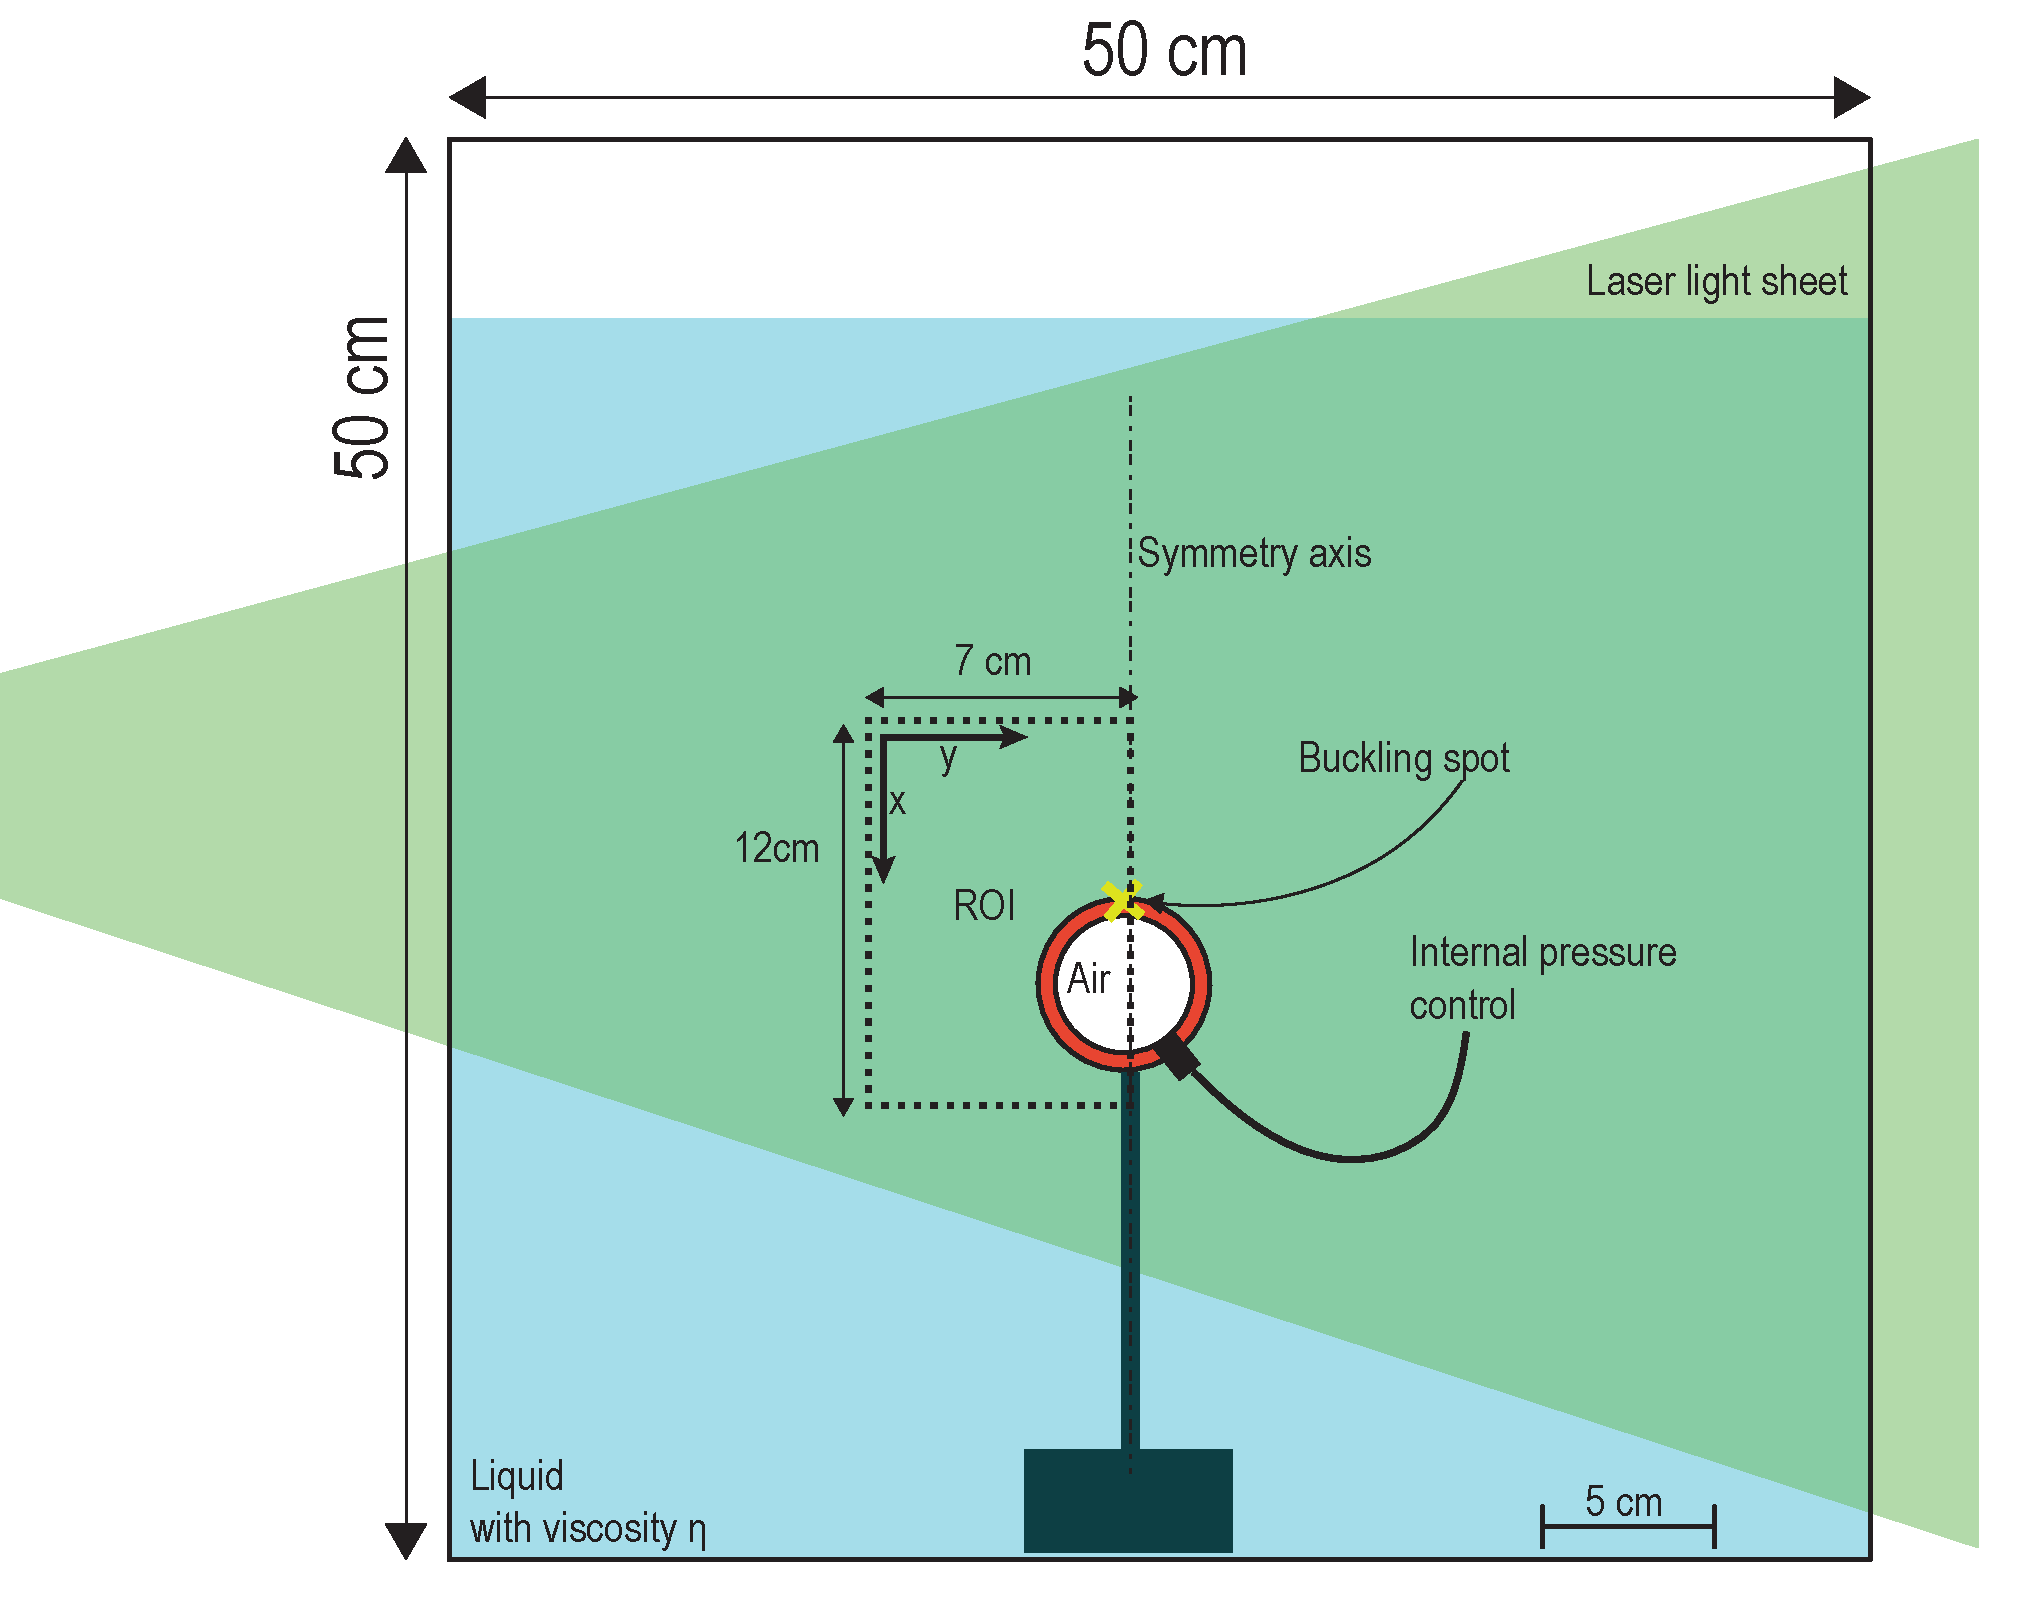
\includegraphics[width=\textwidth]{figures/Chapter_1/piv_experimental_setup.pdf}
	\caption{Schematics of the PIV experimental setup}
	\label{fig:piv_schematics}
\end{figure}

\subsection{Equipment}
\paragraph{}
The complexity of the flow generated by the buckling and unbuckling phases lies in its highly unsteady nature. When the instability occurs, the flow goes from a rest state to an unsteady state with different relevant characteristic times which span from the $10^{-5}$ s to few seconds.\\ This is why it was critical to choose the right equipment to study it.
\subsubsection{Laser source, light sheet generator and camera}

In order to investigate the short unsteady flow generated during the deflation and re-inflation, a good temporal resolution is needed to capture the physics of the flow. Two optical systems were considered: A \textbf{high-frequency}\footnote{Common pulsed laser sources such as "`Nd:YAG-based"' have a freqeuncy that ranges between 10 and 50 Hz, which is the major downside of Nd:YAG-based systems when performing time-resolved experiments except for very low-speed flows ($v < 0.2$m/s)\cite{PIV_springer}.} pulsed laser system coupled with a triggable camera, and a continuous laser source coupled with a high-speed camera. The latter system was chosen, due to the availability of the equipment at the "`LEGI"' laboratory.
A $5$ $W$ continuous laser source which emits at $532$ nm wavelength was used. It was necessary to operate at such a high power, in order to collect a satisfying light scattering from the tracer particles during a period of $50$ $\mu m$.\\
To generate a thin light sheet, the laser source is guided inside an optical arm which is basically an assembly of hollow metal tubes provided with mirrors at the joints allowing to direct the beam (see fig.\ref{fig:optical_system_PIV}). The optical arm ends with an optical system composed of a set of lenses that generate the thin light sheet, allowing the possibility to rotate and to thin the resulting light sheet. It was positioned at 1m from the position of the spherical shell, to have a homogenous thickness of the light sheet.\\ 
\begin{figure}[H]%
	\centering%
	\includegraphics[width=0.75\textwidth]{figures/Chapter_1/optical_system_PIV.pdf}
	\caption{Picture of the laser and optical system used for the PIV measurements}
	\label{fig:optical_system_PIV}
\end{figure}
A high-frequency camera Phantom\textcopyright V2511 was used to capture the PIV image frames, its main characteristics are:
\begin{itemize}
	\item Resolution: One Megapixel, 1280x800.
	\item Full resolution speed: 25000 frame per second (FPS).
	\item Sensor: CMOS sensor with 28 $\mu$m pixel size, 12-bit depth gray-scale colors.
\end{itemize}
The camera was coupled with a macro lens "`Milvus 2/100M"' ZEISS in order to have a satisfying spatial resolution, and was positioned at 45 cm from the shell, providing a field of view of 12cm x 7cm.
\subsubsection{Tracer particles}
The tracer particles used for the PIV measurements are spherical hollow glass particles coated with silver, with a density of $1050$ Kg/$m^3$, with a diameter ranging between $10-30$ $\mu$m. To choose the right tracer particles, we minimized the slip velocity which corresponds to the difference between the particle velocity and the flow velocity\cite{PIV_springer}, expressed as:
\begin{equation*}
v_p−U = \frac{2}{9}\frac{a^2 (\rho_p−\rho_f )}{\mu}\frac{dv_p}{dt}
\label{eq:}
\end{equation*}  
Where $a$ corresponds to the diameter of the particle, $\rho_p$ to the density of the particle,$\rho_f$ to the density of the fluid, $\mu$ to the viscosity of the fluid and $\frac{dv_p}{dt}$ to the acceleration of the particle.
To minimize this expression, we focused on minimizing the diameter and the difference of densities. In the case of water, max($v_p−U$)$=15.10^{-5}$ m/s, and in the case of glycerol, max($v_p−U$)$=7.5.10^{-6}$ m/s, these values are negligible compared to the experimental velocity range $U \in [0.1,3]$ m/s.\\
Another requirement to take into account when choosing the seeding particles is that they should scatter enough light in order to be visible. The particle scattering cross section depends on the particle diameter $a$, the wavelength of the light $\lambda$, and the refractive index of the particle (relative
to the refractive index of the surrounding medium)\cite{PIV_springer}. In order to maximize the light scattering, we chose a particles with a diameter ($a >\lambda$) in order to be in the Mie regime, which yields a scattering cross section roughly proportional to $a^2$\footnote{when the particle diameter becomes less than the wavelength of light, the scattering cross section is proportional to $a^4$}. We also chose particles made of hollow glass coated with silver, which increase the intensity of the reflected light by an order of magnitude compared to solid beads such as polystyrene\cite{PIV_Wiley}.\\
\subsection{Experimental protocol}
\paragraph{Laser sheet and camera alignment}
PIV measurement were conducted in water and glycerol. Each time we fill the tank with a new liquid, preliminary steps were performed to set the camera optical axis normal to the light sheet plane. To do so, a low power light sheet is turned on,  and a uniformly spaced dot grid is introduced in the liquid. We bring the grid tangentially to the light sheet, then we focus the camera on the grid and we tune its position to have all the dots of the grid in the focus plane, which means that the camera optical axis is normal to the light sheet. We capture an image frame of the grid used later to calibrate distance conversion.
\paragraph{Seeding}
A solution of $10$ g of tracer particles diluted in $100$ ml of water is prepared to seed the 110 l of liquid present in the tank. This yields roughly 200 particles in an area of 100x100 px. A surfactant is added to the solution to decrease the presence of clusters of particles, by reducing their cohesiveness.\\
The seeding solution is poured in the liquid, along the light sheet plane, then it is mixed locally to homogenize the distribution along the plane.\\ 
\paragraph{}
The experimental protocol is fairly simple and follows these steps for each shell:
\begin{enumerate}
	\item The shell is attached to the fixed support and positioned in a way that the sheet line crosses it in the middle. It is also positioned along the light sheet plane so that only half of the shell is visible to the camera in the ROI frame shown in figure \ref{fig:piv_schematics}. This strategy is adopted to increase the spatial resolution, by assuming an axis symmetry of the flow.
	\item When the flow comes back to rest, the laser sheet is turned on, operating with a source at 3W.
	\item Pressure inside the shell is dropped to the critical pressure of buckling and the camera is triggered just before the instability, operating at 20khz. The image frames are then saved into the computer.
	\item Pressure inside the shell is increased to the critical pressure of unbuckling and the camera is triggered just before the instability, operating at 20khz.
\end{enumerate}
 \paragraph{Note}
In water, experiments are also conducted at 1khz, because the flow continues to evolve after the end of the deformations.


\subsection{Image processing}
\paragraph{}
A commercial software "`Lavision"'\textcopyright "`Davis"' was used to extract the time resolved velocity fields from the recorded image frames. The processing principle is based on cross-correlation analysis of the particle-image patterns in small sub-domains between two successive image frames. The following steps summarize the basic operations performed to extract the velocity field:
\begin{enumerate}
	\item To convert the pixel space into the physical space, a calibration is performed by using the dot grid image captured at the beginning of the experiments.
	\item Images set is imported into the software and the time step is set.
	\item Since the geometry of the shells evolves through time, a dynamical masking of the non-fluid domain is performed by using a sequence of image treatment operations to identify and mask the deforming shell, followed by a geometrical masking of the rigid non-fluid domain.
	\item Then, cross-correlation analysis parameters are entered, setting the size of the interrogation windows, the number of passes to perform in order to increase precision\footnote{Perform analysis on large-sized interrogation windows and re-iterate on smaller ones, with window overlapping.}.
	\item Finally, a post-processing step is performed to filter aberrant vectors, using statistical tools and thresholds specified by the user.
\end{enumerate}
Details about the image processing settings can be found in the appendix \ref{AppendixA}.

\section{Summary of the experimental setups}
\paragraph{}
The purpose of this study is to investigate swimming of a spherical shell encapsulating a volume of air. The swimming mechanics rely on the buckling instability which is triggered by submitting the elastic shell to pressure cycles. When pressure is increased, the shell is compressed isotropically, until reaching a critical pressure where the symmetry is broken through an instability called buckling. The shape of the shell transits brutally from a spherical configuration to a concave configuration, with a drastic change in the volume. When the pressure is decreased the shell re-inflates following shape configurations not encountered before, until reaching a critical pressure where it jumps back to a spherical shape configuration through another instability called un-buckling. The shape configuration path resulting from the pressure cycle presents an hysteresis in the deformation space. This condition is necessary to achieve swimming in flows where the viscous forces dominate. Further more, the swiftness of the deformations during the buckling and unbuckling phases suggests that the resulting flow might exhibit inertial effects.
\paragraph{}
To study the swimming mechanics, and more precisely the instability dynamics and in which manner it affects the surrounding flow, spherical shells were cast in elastomer materials, and three experimental setups were developed:

\paragraph{Spring experiment}
The purpose of this experiment is to quantify the thrust generated during the buckling and unbuckling phases when the pressure cycle is imposed externally, using a force sensor. The capsule is attached to a spring and immersed in a tank filled with a Newtonian liquid characterized with a density $\rho$ and a viscosity $\mu$. The spring plays the role of a force sensor and prevents the spherical shell from floating to the surface due to buoyancy effects.  The buckling spot is directed in the vertical direction, to get a 1-D displacement. The shell is submitted to external pressure cycles, and images are recorded capturing the shell's shape and the spring position, which gives access to all the forces involved in the phenomenon, through extensive image treatment. Two parameters were explored, the relative thickness $\frac{d}{R}$ which translates the shell's ability to store elastic energy, and the viscosity and density of the surrounding medium.

\paragraph{Frictionless rail experiment}
The purpose of this experiment is to characterize the swimming induced by the shell deformation.
The shell was attached to a support itself mounted on an air bearing frictionless rail, and immersed in a fluid which is a water/glycerol or water/Ucon oil (Dow chemicals) mixture. The air volume it encloses was connected to a pressure controller through a flexible pipe, allowing cycles in the pressure drop $\Delta P$ with an amplitude $\pm 1$ bar. In order to ensure a 1-D problem, the shell was oriented so that the buckling spot pointed in a direction parallel to the rail. Position of the moving support on the rail and shell deformation were recorded using a fast camera. Four parameters were explored: first, the relative thickness $\frac{d}{R}$. second, the viscosity of the surrounding medium. Third, the effect of the dissipation in the material. And finally, the proximity to the wall.

\paragraph{PIV measurements}
To understand the evolution of the displacement obtained in the deflating and the re-inflating of the spherical shell, and how it is affected by the viscosity of the surrounding medium, it was necessary to first, characterize the flow generated during both phases, and to understand how this flow changes with the fluid viscosity. To do so, particle image velocimetry measurements were conducted, by attaching the shell to a rigid support and immerse it in a large tank filled with either water or glycerol. The fluid is seeded with tracer particles, which are lighten by a laser thin sheet. Images are recorded during the buckling and unbuckling phases, using a high-speed camera, positioned in the direction normal to the light sheet. Four parameters were explored: first, the relative thickness $\frac{d}{R}$. Second, the viscosity of the surrounding medium. Third, the effect of the dissipation in the material. And finally, the proximity to the wall.

\paragraph{}
This sums up the material and methods developed for this study. In the next chapter, the different results extracted from the three experimental setups will be exposed and discussed. 







  

  
 



 